% Options for packages loaded elsewhere
\PassOptionsToPackage{unicode}{hyperref}
\PassOptionsToPackage{hyphens}{url}
\PassOptionsToPackage{dvipsnames,svgnames,x11names}{xcolor}
%
\documentclass[
]{article}

\usepackage{amsmath,amssymb}
\usepackage{iftex}
\ifPDFTeX
  \usepackage[T1]{fontenc}
  \usepackage[utf8]{inputenc}
  \usepackage{textcomp} % provide euro and other symbols
\else % if luatex or xetex
  \usepackage{unicode-math}
  \defaultfontfeatures{Scale=MatchLowercase}
  \defaultfontfeatures[\rmfamily]{Ligatures=TeX,Scale=1}
\fi
\usepackage{lmodern}
\ifPDFTeX\else  
    % xetex/luatex font selection
\fi
% Use upquote if available, for straight quotes in verbatim environments
\IfFileExists{upquote.sty}{\usepackage{upquote}}{}
\IfFileExists{microtype.sty}{% use microtype if available
  \usepackage[]{microtype}
  \UseMicrotypeSet[protrusion]{basicmath} % disable protrusion for tt fonts
}{}
\makeatletter
\@ifundefined{KOMAClassName}{% if non-KOMA class
  \IfFileExists{parskip.sty}{%
    \usepackage{parskip}
  }{% else
    \setlength{\parindent}{0pt}
    \setlength{\parskip}{6pt plus 2pt minus 1pt}}
}{% if KOMA class
  \KOMAoptions{parskip=half}}
\makeatother
\usepackage{xcolor}
\setlength{\emergencystretch}{3em} % prevent overfull lines
\setcounter{secnumdepth}{-\maxdimen} % remove section numbering
% Make \paragraph and \subparagraph free-standing
\makeatletter
\ifx\paragraph\undefined\else
  \let\oldparagraph\paragraph
  \renewcommand{\paragraph}{
    \@ifstar
      \xxxParagraphStar
      \xxxParagraphNoStar
  }
  \newcommand{\xxxParagraphStar}[1]{\oldparagraph*{#1}\mbox{}}
  \newcommand{\xxxParagraphNoStar}[1]{\oldparagraph{#1}\mbox{}}
\fi
\ifx\subparagraph\undefined\else
  \let\oldsubparagraph\subparagraph
  \renewcommand{\subparagraph}{
    \@ifstar
      \xxxSubParagraphStar
      \xxxSubParagraphNoStar
  }
  \newcommand{\xxxSubParagraphStar}[1]{\oldsubparagraph*{#1}\mbox{}}
  \newcommand{\xxxSubParagraphNoStar}[1]{\oldsubparagraph{#1}\mbox{}}
\fi
\makeatother

\usepackage{color}
\usepackage{fancyvrb}
\newcommand{\VerbBar}{|}
\newcommand{\VERB}{\Verb[commandchars=\\\{\}]}
\DefineVerbatimEnvironment{Highlighting}{Verbatim}{commandchars=\\\{\}}
% Add ',fontsize=\small' for more characters per line
\usepackage{framed}
\definecolor{shadecolor}{RGB}{241,243,245}
\newenvironment{Shaded}{\begin{snugshade}}{\end{snugshade}}
\newcommand{\AlertTok}[1]{\textcolor[rgb]{0.68,0.00,0.00}{#1}}
\newcommand{\AnnotationTok}[1]{\textcolor[rgb]{0.37,0.37,0.37}{#1}}
\newcommand{\AttributeTok}[1]{\textcolor[rgb]{0.40,0.45,0.13}{#1}}
\newcommand{\BaseNTok}[1]{\textcolor[rgb]{0.68,0.00,0.00}{#1}}
\newcommand{\BuiltInTok}[1]{\textcolor[rgb]{0.00,0.23,0.31}{#1}}
\newcommand{\CharTok}[1]{\textcolor[rgb]{0.13,0.47,0.30}{#1}}
\newcommand{\CommentTok}[1]{\textcolor[rgb]{0.37,0.37,0.37}{#1}}
\newcommand{\CommentVarTok}[1]{\textcolor[rgb]{0.37,0.37,0.37}{\textit{#1}}}
\newcommand{\ConstantTok}[1]{\textcolor[rgb]{0.56,0.35,0.01}{#1}}
\newcommand{\ControlFlowTok}[1]{\textcolor[rgb]{0.00,0.23,0.31}{\textbf{#1}}}
\newcommand{\DataTypeTok}[1]{\textcolor[rgb]{0.68,0.00,0.00}{#1}}
\newcommand{\DecValTok}[1]{\textcolor[rgb]{0.68,0.00,0.00}{#1}}
\newcommand{\DocumentationTok}[1]{\textcolor[rgb]{0.37,0.37,0.37}{\textit{#1}}}
\newcommand{\ErrorTok}[1]{\textcolor[rgb]{0.68,0.00,0.00}{#1}}
\newcommand{\ExtensionTok}[1]{\textcolor[rgb]{0.00,0.23,0.31}{#1}}
\newcommand{\FloatTok}[1]{\textcolor[rgb]{0.68,0.00,0.00}{#1}}
\newcommand{\FunctionTok}[1]{\textcolor[rgb]{0.28,0.35,0.67}{#1}}
\newcommand{\ImportTok}[1]{\textcolor[rgb]{0.00,0.46,0.62}{#1}}
\newcommand{\InformationTok}[1]{\textcolor[rgb]{0.37,0.37,0.37}{#1}}
\newcommand{\KeywordTok}[1]{\textcolor[rgb]{0.00,0.23,0.31}{\textbf{#1}}}
\newcommand{\NormalTok}[1]{\textcolor[rgb]{0.00,0.23,0.31}{#1}}
\newcommand{\OperatorTok}[1]{\textcolor[rgb]{0.37,0.37,0.37}{#1}}
\newcommand{\OtherTok}[1]{\textcolor[rgb]{0.00,0.23,0.31}{#1}}
\newcommand{\PreprocessorTok}[1]{\textcolor[rgb]{0.68,0.00,0.00}{#1}}
\newcommand{\RegionMarkerTok}[1]{\textcolor[rgb]{0.00,0.23,0.31}{#1}}
\newcommand{\SpecialCharTok}[1]{\textcolor[rgb]{0.37,0.37,0.37}{#1}}
\newcommand{\SpecialStringTok}[1]{\textcolor[rgb]{0.13,0.47,0.30}{#1}}
\newcommand{\StringTok}[1]{\textcolor[rgb]{0.13,0.47,0.30}{#1}}
\newcommand{\VariableTok}[1]{\textcolor[rgb]{0.07,0.07,0.07}{#1}}
\newcommand{\VerbatimStringTok}[1]{\textcolor[rgb]{0.13,0.47,0.30}{#1}}
\newcommand{\WarningTok}[1]{\textcolor[rgb]{0.37,0.37,0.37}{\textit{#1}}}

\providecommand{\tightlist}{%
  \setlength{\itemsep}{0pt}\setlength{\parskip}{0pt}}\usepackage{longtable,booktabs,array}
\usepackage{calc} % for calculating minipage widths
% Correct order of tables after \paragraph or \subparagraph
\usepackage{etoolbox}
\makeatletter
\patchcmd\longtable{\par}{\if@noskipsec\mbox{}\fi\par}{}{}
\makeatother
% Allow footnotes in longtable head/foot
\IfFileExists{footnotehyper.sty}{\usepackage{footnotehyper}}{\usepackage{footnote}}
\makesavenoteenv{longtable}
\usepackage{graphicx}
\makeatletter
\def\maxwidth{\ifdim\Gin@nat@width>\linewidth\linewidth\else\Gin@nat@width\fi}
\def\maxheight{\ifdim\Gin@nat@height>\textheight\textheight\else\Gin@nat@height\fi}
\makeatother
% Scale images if necessary, so that they will not overflow the page
% margins by default, and it is still possible to overwrite the defaults
% using explicit options in \includegraphics[width, height, ...]{}
\setkeys{Gin}{width=\maxwidth,height=\maxheight,keepaspectratio}
% Set default figure placement to htbp
\makeatletter
\def\fps@figure{htbp}
\makeatother

\usepackage{booktabs}
\usepackage{longtable}
\usepackage{array}
\usepackage{multirow}
\usepackage{wrapfig}
\usepackage{float}
\usepackage{colortbl}
\usepackage{pdflscape}
\usepackage{tabu}
\usepackage{threeparttable}
\usepackage{threeparttablex}
\usepackage[normalem]{ulem}
\usepackage{makecell}
\usepackage{xcolor}
\makeatletter
\@ifpackageloaded{caption}{}{\usepackage{caption}}
\AtBeginDocument{%
\ifdefined\contentsname
  \renewcommand*\contentsname{Table of contents}
\else
  \newcommand\contentsname{Table of contents}
\fi
\ifdefined\listfigurename
  \renewcommand*\listfigurename{List of Figures}
\else
  \newcommand\listfigurename{List of Figures}
\fi
\ifdefined\listtablename
  \renewcommand*\listtablename{List of Tables}
\else
  \newcommand\listtablename{List of Tables}
\fi
\ifdefined\figurename
  \renewcommand*\figurename{Figure}
\else
  \newcommand\figurename{Figure}
\fi
\ifdefined\tablename
  \renewcommand*\tablename{Table}
\else
  \newcommand\tablename{Table}
\fi
}
\@ifpackageloaded{float}{}{\usepackage{float}}
\floatstyle{ruled}
\@ifundefined{c@chapter}{\newfloat{codelisting}{h}{lop}}{\newfloat{codelisting}{h}{lop}[chapter]}
\floatname{codelisting}{Listing}
\newcommand*\listoflistings{\listof{codelisting}{List of Listings}}
\makeatother
\makeatletter
\makeatother
\makeatletter
\@ifpackageloaded{caption}{}{\usepackage{caption}}
\@ifpackageloaded{subcaption}{}{\usepackage{subcaption}}
\makeatother

\ifLuaTeX
  \usepackage{selnolig}  % disable illegal ligatures
\fi
\usepackage{bookmark}

\IfFileExists{xurl.sty}{\usepackage{xurl}}{} % add URL line breaks if available
\urlstyle{same} % disable monospaced font for URLs
\hypersetup{
  pdftitle={Analytics Report Shell},
  pdfauthor={Dillon Labonte},
  colorlinks=true,
  linkcolor={blue},
  filecolor={Maroon},
  citecolor={Blue},
  urlcolor={Blue},
  pdfcreator={LaTeX via pandoc}}


\title{Analytics Report Shell}
\author{Dillon Labonte}
\date{February 16, 2025}

\begin{document}
\maketitle

\renewcommand*\contentsname{Table of contents}
{
\hypersetup{linkcolor=}
\setcounter{tocdepth}{3}
\tableofcontents
}

\begin{Shaded}
\begin{Highlighting}[]
\CommentTok{\# including necessary libraries}
\FunctionTok{library}\NormalTok{(tidyverse)}
\FunctionTok{library}\NormalTok{(tidymodels)}
\FunctionTok{library}\NormalTok{(patchwork)}
\FunctionTok{library}\NormalTok{(kableExtra)}

\CommentTok{\# styling}
\FunctionTok{options}\NormalTok{(}\AttributeTok{kable\_styling\_bootstrap\_options =} \FunctionTok{c}\NormalTok{(}\StringTok{"hover"}\NormalTok{, }\StringTok{"striped"}\NormalTok{))}
\FunctionTok{theme\_set}\NormalTok{(}\FunctionTok{theme\_bw}\NormalTok{(}\AttributeTok{base\_size =} \DecValTok{14}\NormalTok{))}

\CommentTok{\# read in data and clean up column names}
\NormalTok{data }\OtherTok{\textless{}{-}} \FunctionTok{read\_csv}\NormalTok{(}\StringTok{"energy\_dataset.csv"}\NormalTok{)}
\FunctionTok{names}\NormalTok{(data) }\OtherTok{\textless{}{-}}\NormalTok{ janitor}\SpecialCharTok{::}\FunctionTok{make\_clean\_names}\NormalTok{(}\FunctionTok{names}\NormalTok{(data))}

\CommentTok{\# adding generation\_total column to data set}
\NormalTok{data }\OtherTok{\textless{}{-}}\NormalTok{ data }\SpecialCharTok{|\textgreater{}}
  \FunctionTok{mutate}\NormalTok{(}\AttributeTok{generation\_total =}\NormalTok{ generation\_biomass }\SpecialCharTok{+}\NormalTok{ generation\_fossil\_brown\_coal\_lignite }\SpecialCharTok{+}\NormalTok{ generation\_fossil\_coal\_derived\_gas }\SpecialCharTok{+}\NormalTok{ generation\_fossil\_gas }\SpecialCharTok{+}\NormalTok{ generation\_fossil\_hard\_coal }\SpecialCharTok{+}\NormalTok{ generation\_fossil\_oil }\SpecialCharTok{+}\NormalTok{ generation\_fossil\_oil\_shale }\SpecialCharTok{+}\NormalTok{ generation\_fossil\_peat }\SpecialCharTok{+}\NormalTok{ generation\_geothermal }\SpecialCharTok{+}\NormalTok{ generation\_hydro\_pumped\_storage\_consumption }\SpecialCharTok{+}\NormalTok{ generation\_hydro\_run\_of\_river\_and\_poundage }\SpecialCharTok{+}\NormalTok{ generation\_hydro\_water\_reservoir }\SpecialCharTok{+}\NormalTok{ generation\_marine }\SpecialCharTok{+}\NormalTok{ generation\_nuclear }\SpecialCharTok{+}\NormalTok{ generation\_other }\SpecialCharTok{+}\NormalTok{ generation\_other\_renewable }\SpecialCharTok{+}\NormalTok{ generation\_solar }\SpecialCharTok{+}\NormalTok{ generation\_waste }\SpecialCharTok{+}\NormalTok{ generation\_wind\_offshore }\SpecialCharTok{+}\NormalTok{ generation\_wind\_onshore)}

\CommentTok{\# adding renewable\_generation\_total column to data set}
\NormalTok{data }\OtherTok{\textless{}{-}}\NormalTok{ data }\SpecialCharTok{|\textgreater{}}
  \FunctionTok{mutate}\NormalTok{(}\AttributeTok{renewable\_generation\_total =}\NormalTok{ generation\_biomass }\SpecialCharTok{+}\NormalTok{ generation\_geothermal }\SpecialCharTok{+}\NormalTok{ generation\_hydro\_run\_of\_river\_and\_poundage }\SpecialCharTok{+}\NormalTok{ generation\_hydro\_water\_reservoir }\SpecialCharTok{+}\NormalTok{ generation\_hydro\_pumped\_storage\_consumption }\SpecialCharTok{+}\NormalTok{ generation\_marine }\SpecialCharTok{+}\NormalTok{ generation\_other\_renewable }\SpecialCharTok{+}\NormalTok{ generation\_solar }\SpecialCharTok{+}\NormalTok{ generation\_wind\_offshore }\SpecialCharTok{+}\NormalTok{ generation\_wind\_onshore)}

\CommentTok{\# adding nonrenewable\_generation\_total column to data set}
\NormalTok{data }\OtherTok{\textless{}{-}}\NormalTok{ data }\SpecialCharTok{|\textgreater{}}
  \FunctionTok{mutate}\NormalTok{(}\AttributeTok{nonrenewable\_generation\_total =}\NormalTok{ generation\_fossil\_brown\_coal\_lignite }\SpecialCharTok{+}\NormalTok{ generation\_fossil\_coal\_derived\_gas }\SpecialCharTok{+}\NormalTok{ generation\_fossil\_gas }\SpecialCharTok{+}\NormalTok{ generation\_fossil\_hard\_coal }\SpecialCharTok{+}\NormalTok{ generation\_fossil\_oil }\SpecialCharTok{+}\NormalTok{ generation\_fossil\_oil\_shale }\SpecialCharTok{+}\NormalTok{ generation\_fossil\_peat)}

\CommentTok{\# adding hour\_of\_day column to data set}
\NormalTok{data }\OtherTok{\textless{}{-}}\NormalTok{ data }\SpecialCharTok{|\textgreater{}}
  \FunctionTok{mutate}\NormalTok{(}\AttributeTok{hour\_of\_day =} \FunctionTok{hour}\NormalTok{(time))}

\CommentTok{\# adding month\_of\_year column to data set}
\NormalTok{data }\OtherTok{\textless{}{-}}\NormalTok{ data }\SpecialCharTok{|\textgreater{}}
  \FunctionTok{mutate}\NormalTok{(}\AttributeTok{month\_of\_year =} \FunctionTok{month}\NormalTok{(time, }\AttributeTok{label =} \ConstantTok{TRUE}\NormalTok{, }\AttributeTok{abbr =} \ConstantTok{TRUE}\NormalTok{))}

\CommentTok{\# calculating RMSE of TSO model for price\_day\_ahead}
\NormalTok{tso\_rmse }\OtherTok{\textless{}{-}}\NormalTok{ data }\SpecialCharTok{|\textgreater{}}
  \FunctionTok{rmse}\NormalTok{(price\_day\_ahead, price\_actual)}

\CommentTok{\# split data into training, test, and validation sets}
\FunctionTok{set.seed}\NormalTok{(}\DecValTok{1234567890}\NormalTok{)}
\NormalTok{data\_splits }\OtherTok{\textless{}{-}} \FunctionTok{initial\_split}\NormalTok{(data, }\AttributeTok{prop =} \FloatTok{0.75}\NormalTok{)}

\NormalTok{train }\OtherTok{\textless{}{-}} \FunctionTok{training}\NormalTok{(data\_splits)}
\NormalTok{temp }\OtherTok{\textless{}{-}} \FunctionTok{testing}\NormalTok{(data\_splits)}

\FunctionTok{set.seed}\NormalTok{(}\DecValTok{11111}\NormalTok{)}
\NormalTok{test\_splits }\OtherTok{\textless{}{-}} \FunctionTok{initial\_split}\NormalTok{(temp, }\AttributeTok{prop =} \FloatTok{0.5}\NormalTok{)}
\NormalTok{validation }\OtherTok{\textless{}{-}} \FunctionTok{training}\NormalTok{(test\_splits)}
\NormalTok{test }\OtherTok{\textless{}{-}} \FunctionTok{testing}\NormalTok{(test\_splits)}
\end{Highlighting}
\end{Shaded}

\begin{Shaded}
\begin{Highlighting}[]
\CommentTok{\# creating a predictors data set to use for model building}
\NormalTok{predictors }\OtherTok{\textless{}{-}}\NormalTok{ train }\SpecialCharTok{|\textgreater{}}
  \FunctionTok{select}\NormalTok{(}\SpecialCharTok{{-}}\FunctionTok{c}\NormalTok{(time, generation\_hydro\_pumped\_storage\_aggregated, forecast\_wind\_offshore\_eday\_ahead, total\_load\_actual, price\_day\_ahead, generation\_total, renewable\_generation\_total, nonrenewable\_generation\_total))}
\end{Highlighting}
\end{Shaded}

\subsection{Statement of Purpose}\label{statement-of-purpose}

This project seeks to develop a regression model to predict day ahead
electrical power prices by analyzing energy generation, demand, and
weather forecasts. These predictions support grid operators, producers,
and consumers in maintaining grid stability and optimizing energy use,
especially as renewable energy sources grow in popularity.

\subsection{Executive Summary}\label{executive-summary}

In order to assist grid operators, energy producers, and customers in
making well-informed decisions, this project aimed to predict
electricity prices for the following day. Reliable pricing predictions
reduce issues brought on by the fluctuations of renewable energy
sources, improve grid stability, and optimize generation and
consumption. Using an extensive dataset that included hourly electricity
prices, generation, demand, and weather data from 2015 to 2018, the
project focused on Spain's electrical grid, with implications in other
energy grids around the world.

A number of predictive models were constructed and assessed. The TSO
model, a baseline model constructed by ENTSOE, produced a high RMSE of
13.25. We created three models in response: linear regression, random
forest, and extreme gradient boosting. Hyper parameter tuning was used
to maximize the predictability of these models. With an RMSE of 3.44 on
validation data, the extreme gradient boosting model performed the best,
allowing predictions to be within plus or minus \$7 of actual prices.

The results of this analysis shows that extreme gradient boosting and
other advanced machine learning models provide significant improvements
in prediction accuracy. These results highlight how regression can
improve grid sustainability and reliability in a market driven by ever
increasing renewable energy generation. These results offer useful
insights in other global electrical grids.

\subsection{Introduction}\label{introduction}

The price of electrical power is a constantly changing variable that
profoundly impacts society. Being able to predict electrical power
prices a day in advance would allow for increased grid stability which
is necessary to maintain a delicate balance of electrical supply and
demand that the grid requires. These predictions allow producers of
electricity to decide how much power to produce and when, and industrial
consumers to decide when to use power for energy intensive processes.

In this day and age renewable energies are becoming more popular and
their power production and usage is ever increasing. However, renewable
energy sources are variable and often rely on weather conditions.
Accurate predictions of day ahead prices will allow grid operators to
deploy backup power sources, such as fossil fuels, when needed during
renewable energy fluctuations.

This project aims to build a regression model to predict the electrical
power prices a day in advance by analyzing generation, demand, and
weather forecasts. These predictions support grid operators, producers,
and consumers in their decision making, improving the reliability and
sustainability of the electrical energy market.

This project focuses on Spain's electrical grid with hourly data over
the course of 4 years, from 2015 through 2018. Insights gained from this
analysis of Spain's grid will be useful when considering electrical
grids of other countries that are also incorporating large scale
renewable energy generation.

\subsection{Exploratory Data Analysis}\label{exploratory-data-analysis}

This data set was obtained from the European Network of Transmission
System Operators of Electricity (ENTSOE) {[}1{]}. The transmission
system operator (TSO) uses models to forecast day ahead electrical load
and electricity prices. Let's look at the root mean squared error (RMSE)
of the TSO model predictions for day ahead price, compared to the actual
price.

\begin{Shaded}
\begin{Highlighting}[]
\NormalTok{tso\_rmse }\SpecialCharTok{|\textgreater{}}
  \FunctionTok{kable}\NormalTok{() }\SpecialCharTok{|\textgreater{}}
  \FunctionTok{kable\_styling}\NormalTok{()}
\end{Highlighting}
\end{Shaded}

\begin{longtable*}[t]{llr}
\toprule
.metric & .estimator & .estimate\\
\midrule
rmse & standard & 13.24986\\
\bottomrule
\end{longtable*}

This RMSE is quite bad. This indicates that roughly 95\% of the true day
ahead prices will fall within 2 RMSEs, or about \$26, of the true value.
This is on the same order of magnitude as the electrical prices, often
in the \$50 or \$60 range.

Let's look at the first 6 rows of our dataset to get an idea of what
we're dealing with before making models.

\begin{Shaded}
\begin{Highlighting}[]
\NormalTok{train }\SpecialCharTok{|\textgreater{}}
  \FunctionTok{head}\NormalTok{() }\SpecialCharTok{|\textgreater{}}
  \FunctionTok{kable}\NormalTok{() }\SpecialCharTok{|\textgreater{}}
  \FunctionTok{kable\_styling}\NormalTok{()}
\end{Highlighting}
\end{Shaded}

\begin{longtable*}[t]{lrrrrrrrrrlrrrrrrrrrrrrlrrrrrrrrrl}
\toprule
time & generation\_biomass & generation\_fossil\_brown\_coal\_lignite & generation\_fossil\_coal\_derived\_gas & generation\_fossil\_gas & generation\_fossil\_hard\_coal & generation\_fossil\_oil & generation\_fossil\_oil\_shale & generation\_fossil\_peat & generation\_geothermal & generation\_hydro\_pumped\_storage\_aggregated & generation\_hydro\_pumped\_storage\_consumption & generation\_hydro\_run\_of\_river\_and\_poundage & generation\_hydro\_water\_reservoir & generation\_marine & generation\_nuclear & generation\_other & generation\_other\_renewable & generation\_solar & generation\_waste & generation\_wind\_offshore & generation\_wind\_onshore & forecast\_solar\_day\_ahead & forecast\_wind\_offshore\_eday\_ahead & forecast\_wind\_onshore\_day\_ahead & total\_load\_forecast & total\_load\_actual & price\_day\_ahead & price\_actual & generation\_total & renewable\_generation\_total & nonrenewable\_generation\_total & hour\_of\_day & month\_of\_year\\
\midrule
2017-11-19 21:00:00 & 336 & 656 & 0 & 11431 & 6745 & 262 & 0 & 0 & 0 & NA & 0 & 499 & 1556 & 0 & 5047 & 56 & 83 & 64 & 256 & 0 & 1806 & 46 & NA & 1824 & 29049 & 29439 & 69.72 & 75.25 & 28797 & 4344 & 19094 & 21 & Nov\\
2015-12-26 05:00:00 & 370 & 0 & 0 & 3929 & 1831 & 162 & 0 & 0 & 0 & NA & 3648 & 461 & 291 & 0 & 7103 & 43 & 69 & 24 & 164 & 0 & 6175 & 1 & NA & 6095 & 19520 & 19631 & 29.02 & 42.17 & 24270 & 11038 & 5922 & 5 & Dec\\
2018-03-12 20:00:00 & 397 & 0 & 0 & 9762 & 5383 & 315 & 0 & 0 & 0 & NA & 0 & 1368 & 5987 & 0 & 5539 & 59 & 99 & 45 & 306 & 0 & 3254 & 16 & NA & 3564 & 34957 & 34759 & 69.89 & 77.92 & 32514 & 11150 & 15460 & 20 & Mar\\
2015-04-30 12:00:00 & 376 & 964 & 0 & 4355 & 5990 & 381 & 0 & 0 & 0 & NA & 170 & 1056 & 2237 & 0 & 4040 & 46 & 76 & 5418 & 179 & 0 & 5833 & 4976 & NA & 5920 & 30136 & 30187 & 49.71 & 64.12 & 31121 & 15166 & 11690 & 12 & Apr\\
2018-08-07 11:00:00 & 367 & 419 & 0 & 4862 & 2884 & 221 & 0 & 0 & 0 & NA & 166 & 1232 & 2268 & 0 & 5970 & 55 & 98 & 5454 & 315 & 0 & 2091 & 5171 & NA & 2287 & 28829 & 28200 & 60.97 & 73.98 & 26402 & 11676 & 8386 & 11 & Aug\\
\addlinespace
2018-07-19 03:00:00 & 361 & 660 & 0 & 4579 & 4718 & 236 & 0 & 0 & 0 & NA & 209 & 1027 & 2655 & 0 & 6008 & 54 & 90 & 645 & 307 & 0 & 2017 & 450 & NA & 2170 & 25284 & 25346 & 61.15 & 64.50 & 23566 & 7004 & 10193 & 3 & Jul\\
\bottomrule
\end{longtable*}

Let's look at the distribution of our actual day ahead prices.

\begin{Shaded}
\begin{Highlighting}[]
\NormalTok{priceDayAheadDistribution }\OtherTok{\textless{}{-}}\NormalTok{ train }\SpecialCharTok{|\textgreater{}}
  \FunctionTok{ggplot}\NormalTok{() }\SpecialCharTok{+}
  \FunctionTok{geom\_histogram}\NormalTok{(}\FunctionTok{aes}\NormalTok{(}\AttributeTok{x =}\NormalTok{ price\_actual, }\AttributeTok{y =} \FunctionTok{after\_stat}\NormalTok{(density)), }\AttributeTok{alpha =} \FloatTok{0.6}\NormalTok{) }\SpecialCharTok{+}
  \FunctionTok{geom\_density}\NormalTok{(}\FunctionTok{aes}\NormalTok{(}\AttributeTok{x =}\NormalTok{ price\_actual), }\AttributeTok{fill =} \StringTok{\textquotesingle{}red\textquotesingle{}}\NormalTok{, }\AttributeTok{alpha =} \FloatTok{0.3}\NormalTok{)}

\NormalTok{priceDayAheadDistribution}
\end{Highlighting}
\end{Shaded}

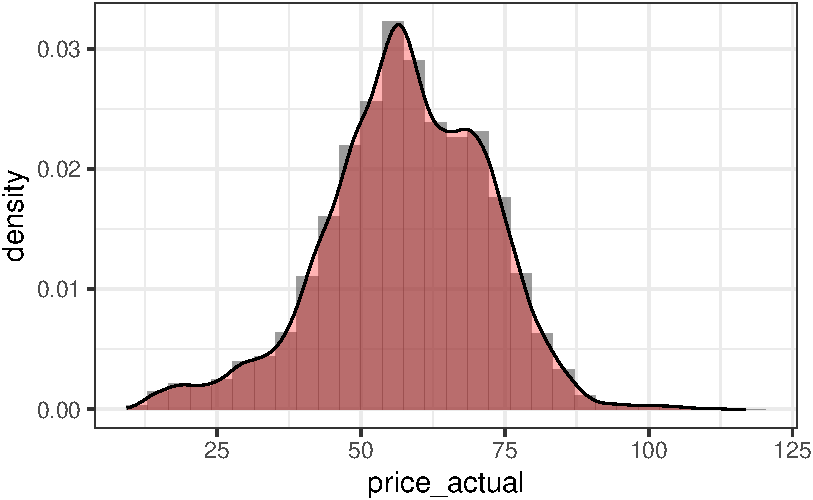
\includegraphics{Analytics_Report_files/figure-pdf/priceDayAheadDistribution-1.pdf}

Our response variable is normally distributed, so we can work with this
response variable without making any changes.

Let's build some plots and see if we can spot any visual trends.

\begin{Shaded}
\begin{Highlighting}[]
\NormalTok{plot1 }\OtherTok{\textless{}{-}}\NormalTok{ train }\SpecialCharTok{|\textgreater{}}
  \FunctionTok{sample\_frac}\NormalTok{(.}\DecValTok{2}\NormalTok{) }\SpecialCharTok{|\textgreater{}}
  \FunctionTok{ggplot}\NormalTok{() }\SpecialCharTok{+}
  \FunctionTok{geom\_point}\NormalTok{(}\FunctionTok{aes}\NormalTok{(}\AttributeTok{x =}\NormalTok{ generation\_total, }\AttributeTok{y =}\NormalTok{ price\_actual), }\AttributeTok{alpha =} \FloatTok{0.3}\NormalTok{) }\SpecialCharTok{+}
  \FunctionTok{geom\_smooth}\NormalTok{(}\FunctionTok{aes}\NormalTok{(}\AttributeTok{x =}\NormalTok{ generation\_total, }\AttributeTok{y =}\NormalTok{ price\_actual))}

\NormalTok{plot2 }\OtherTok{\textless{}{-}}\NormalTok{ train }\SpecialCharTok{|\textgreater{}}
  \FunctionTok{sample\_frac}\NormalTok{(.}\DecValTok{2}\NormalTok{) }\SpecialCharTok{|\textgreater{}}
  \FunctionTok{ggplot}\NormalTok{() }\SpecialCharTok{+}
  \FunctionTok{geom\_point}\NormalTok{(}\FunctionTok{aes}\NormalTok{(}\AttributeTok{x =}\NormalTok{ total\_load\_actual, }\AttributeTok{y =}\NormalTok{ price\_actual), }\AttributeTok{alpha =} \FloatTok{0.3}\NormalTok{) }\SpecialCharTok{+}
  \FunctionTok{geom\_smooth}\NormalTok{(}\FunctionTok{aes}\NormalTok{(}\AttributeTok{x =}\NormalTok{ total\_load\_actual, }\AttributeTok{y =}\NormalTok{ price\_actual))}

\NormalTok{plot3 }\OtherTok{\textless{}{-}}\NormalTok{ train }\SpecialCharTok{|\textgreater{}}
  \FunctionTok{sample\_frac}\NormalTok{(.}\DecValTok{2}\NormalTok{) }\SpecialCharTok{|\textgreater{}}
  \FunctionTok{ggplot}\NormalTok{() }\SpecialCharTok{+}
  \FunctionTok{geom\_point}\NormalTok{(}\FunctionTok{aes}\NormalTok{(}\AttributeTok{x =}\NormalTok{ total\_load\_forecast, }\AttributeTok{y =}\NormalTok{ price\_actual), }\AttributeTok{alpha =} \FloatTok{0.3}\NormalTok{) }\SpecialCharTok{+}
  \FunctionTok{geom\_smooth}\NormalTok{(}\FunctionTok{aes}\NormalTok{(}\AttributeTok{x =}\NormalTok{ total\_load\_forecast, }\AttributeTok{y =}\NormalTok{ price\_actual))}

\NormalTok{plot4 }\OtherTok{\textless{}{-}}\NormalTok{ train }\SpecialCharTok{|\textgreater{}}
  \FunctionTok{sample\_frac}\NormalTok{(.}\DecValTok{2}\NormalTok{) }\SpecialCharTok{|\textgreater{}}
  \FunctionTok{ggplot}\NormalTok{() }\SpecialCharTok{+}
  \FunctionTok{geom\_point}\NormalTok{(}\FunctionTok{aes}\NormalTok{(}\AttributeTok{x =}\NormalTok{ total\_load\_forecast, }\AttributeTok{y =}\NormalTok{ total\_load\_actual), }\AttributeTok{alpha =} \FloatTok{0.3}\NormalTok{) }\SpecialCharTok{+}
  \FunctionTok{geom\_smooth}\NormalTok{(}\FunctionTok{aes}\NormalTok{(}\AttributeTok{x =}\NormalTok{ total\_load\_forecast, }\AttributeTok{y =}\NormalTok{ total\_load\_actual))}

\NormalTok{plot5 }\OtherTok{\textless{}{-}}\NormalTok{ train }\SpecialCharTok{|\textgreater{}}
  \FunctionTok{sample\_frac}\NormalTok{(.}\DecValTok{2}\NormalTok{) }\SpecialCharTok{|\textgreater{}}
  \FunctionTok{ggplot}\NormalTok{() }\SpecialCharTok{+}
  \FunctionTok{geom\_point}\NormalTok{(}\FunctionTok{aes}\NormalTok{(}\AttributeTok{x =}\NormalTok{ price\_day\_ahead, }\AttributeTok{y =}\NormalTok{ price\_actual), }\AttributeTok{alpha =} \FloatTok{0.3}\NormalTok{) }\SpecialCharTok{+}
  \FunctionTok{geom\_smooth}\NormalTok{(}\FunctionTok{aes}\NormalTok{(}\AttributeTok{x =}\NormalTok{ price\_day\_ahead, }\AttributeTok{y =}\NormalTok{ price\_actual))}

\NormalTok{plot6 }\OtherTok{\textless{}{-}}\NormalTok{ train }\SpecialCharTok{|\textgreater{}}
  \FunctionTok{sample\_frac}\NormalTok{(.}\DecValTok{2}\NormalTok{) }\SpecialCharTok{|\textgreater{}}
  \FunctionTok{ggplot}\NormalTok{() }\SpecialCharTok{+}
  \FunctionTok{geom\_point}\NormalTok{(}\FunctionTok{aes}\NormalTok{(}\AttributeTok{x =}\NormalTok{ renewable\_generation\_total, }\AttributeTok{y =}\NormalTok{ price\_actual), }\AttributeTok{alpha =} \FloatTok{0.3}\NormalTok{) }\SpecialCharTok{+}
  \FunctionTok{geom\_smooth}\NormalTok{(}\FunctionTok{aes}\NormalTok{(}\AttributeTok{x =}\NormalTok{ renewable\_generation\_total, }\AttributeTok{y =}\NormalTok{ price\_actual))}

\NormalTok{plot7 }\OtherTok{\textless{}{-}}\NormalTok{ train }\SpecialCharTok{|\textgreater{}}
  \FunctionTok{sample\_frac}\NormalTok{(.}\DecValTok{2}\NormalTok{) }\SpecialCharTok{|\textgreater{}}
  \FunctionTok{ggplot}\NormalTok{() }\SpecialCharTok{+}
  \FunctionTok{geom\_point}\NormalTok{(}\FunctionTok{aes}\NormalTok{(}\AttributeTok{x =}\NormalTok{ nonrenewable\_generation\_total, }\AttributeTok{y =}\NormalTok{ price\_actual), }\AttributeTok{alpha =} \FloatTok{0.3}\NormalTok{) }\SpecialCharTok{+}
  \FunctionTok{geom\_smooth}\NormalTok{(}\FunctionTok{aes}\NormalTok{(}\AttributeTok{x =}\NormalTok{ nonrenewable\_generation\_total, }\AttributeTok{y =}\NormalTok{ price\_actual))}

\NormalTok{plot8 }\OtherTok{\textless{}{-}}\NormalTok{ train}\SpecialCharTok{|\textgreater{}}
  \FunctionTok{sample\_frac}\NormalTok{(.}\DecValTok{2}\NormalTok{) }\SpecialCharTok{|\textgreater{}}
  \FunctionTok{ggplot}\NormalTok{() }\SpecialCharTok{+}
  \FunctionTok{geom\_boxplot}\NormalTok{(}\FunctionTok{aes}\NormalTok{(}\AttributeTok{group =}\NormalTok{ hour\_of\_day, }\AttributeTok{x =}\NormalTok{ hour\_of\_day, }\AttributeTok{y =}\NormalTok{ price\_actual)) }\SpecialCharTok{+}
  \FunctionTok{geom\_smooth}\NormalTok{(}\FunctionTok{aes}\NormalTok{(}\AttributeTok{x =}\NormalTok{ hour\_of\_day, }\AttributeTok{y =}\NormalTok{ price\_actual))}

\NormalTok{plot9 }\OtherTok{\textless{}{-}}\NormalTok{ train}\SpecialCharTok{|\textgreater{}}
  \FunctionTok{sample\_frac}\NormalTok{(.}\DecValTok{2}\NormalTok{) }\SpecialCharTok{|\textgreater{}}
  \FunctionTok{ggplot}\NormalTok{() }\SpecialCharTok{+}
  \FunctionTok{geom\_boxplot}\NormalTok{(}\FunctionTok{aes}\NormalTok{(}\AttributeTok{group =}\NormalTok{ month\_of\_year, }\AttributeTok{x =}\NormalTok{ month\_of\_year, }\AttributeTok{y =}\NormalTok{ price\_actual)) }\SpecialCharTok{+}
  \FunctionTok{geom\_smooth}\NormalTok{(}\FunctionTok{aes}\NormalTok{(}\AttributeTok{x =}\NormalTok{ month\_of\_year, }\AttributeTok{y =}\NormalTok{ price\_actual))}
\end{Highlighting}
\end{Shaded}

The first two plots explore the TSO model predictions of total load and
price, compared to their true values.

\begin{Shaded}
\begin{Highlighting}[]
\NormalTok{plot4 }\SpecialCharTok{/}\NormalTok{ plot5}
\end{Highlighting}
\end{Shaded}

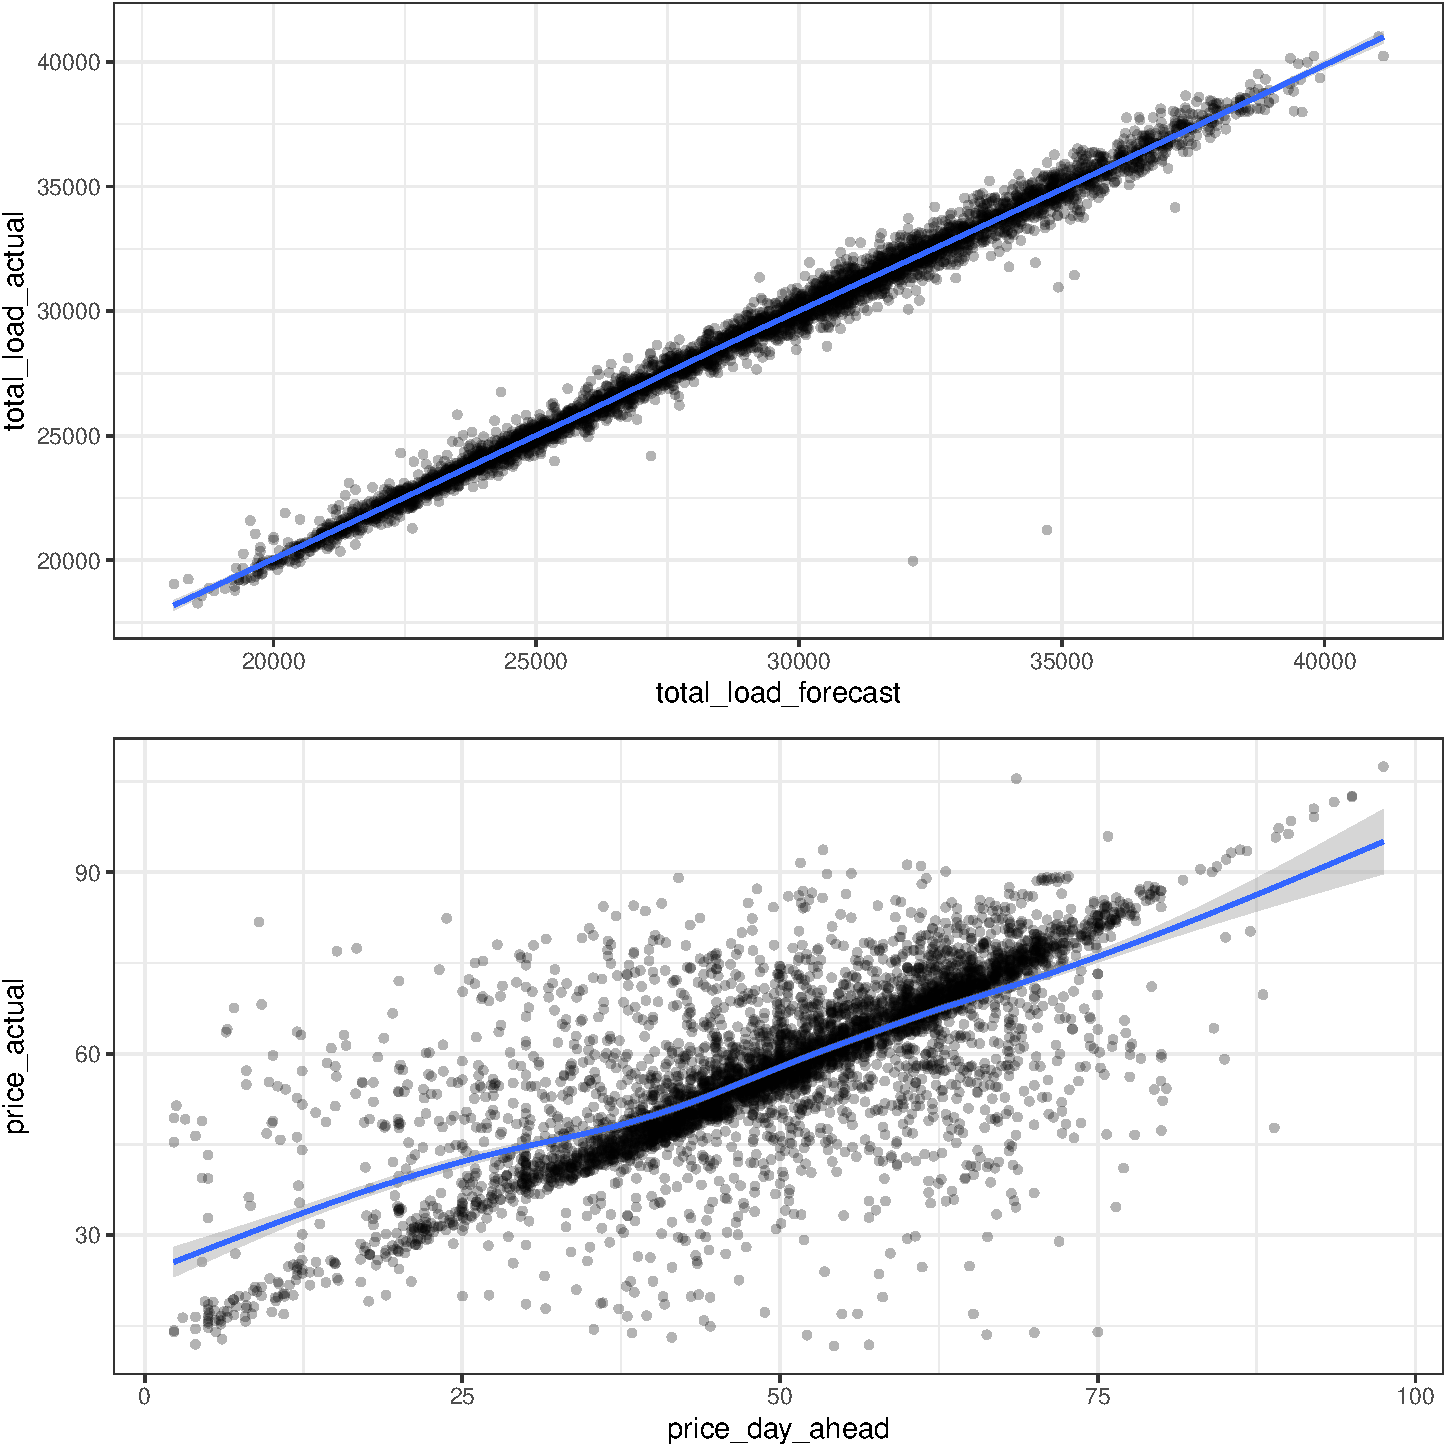
\includegraphics{Analytics_Report_files/figure-pdf/plot45-1.pdf}

In the first plot, the predictions are very accurate and hug the line
\(y = x\), indicating that the model used to predict the total load is
accurate and reliable. However, in the second plot we see that the
predicted prices for the next day are much less accurate. It is clear
they follow some positive relationship, however it is not necessarily
linear. We will try to improve upon this with our models.

The following plots show the affect of generation, and variations of
generation, and how they affect the day ahead price.

\begin{Shaded}
\begin{Highlighting}[]
\NormalTok{plot1 }\SpecialCharTok{/}\NormalTok{ plot6 }\SpecialCharTok{/}\NormalTok{ plot7}
\end{Highlighting}
\end{Shaded}

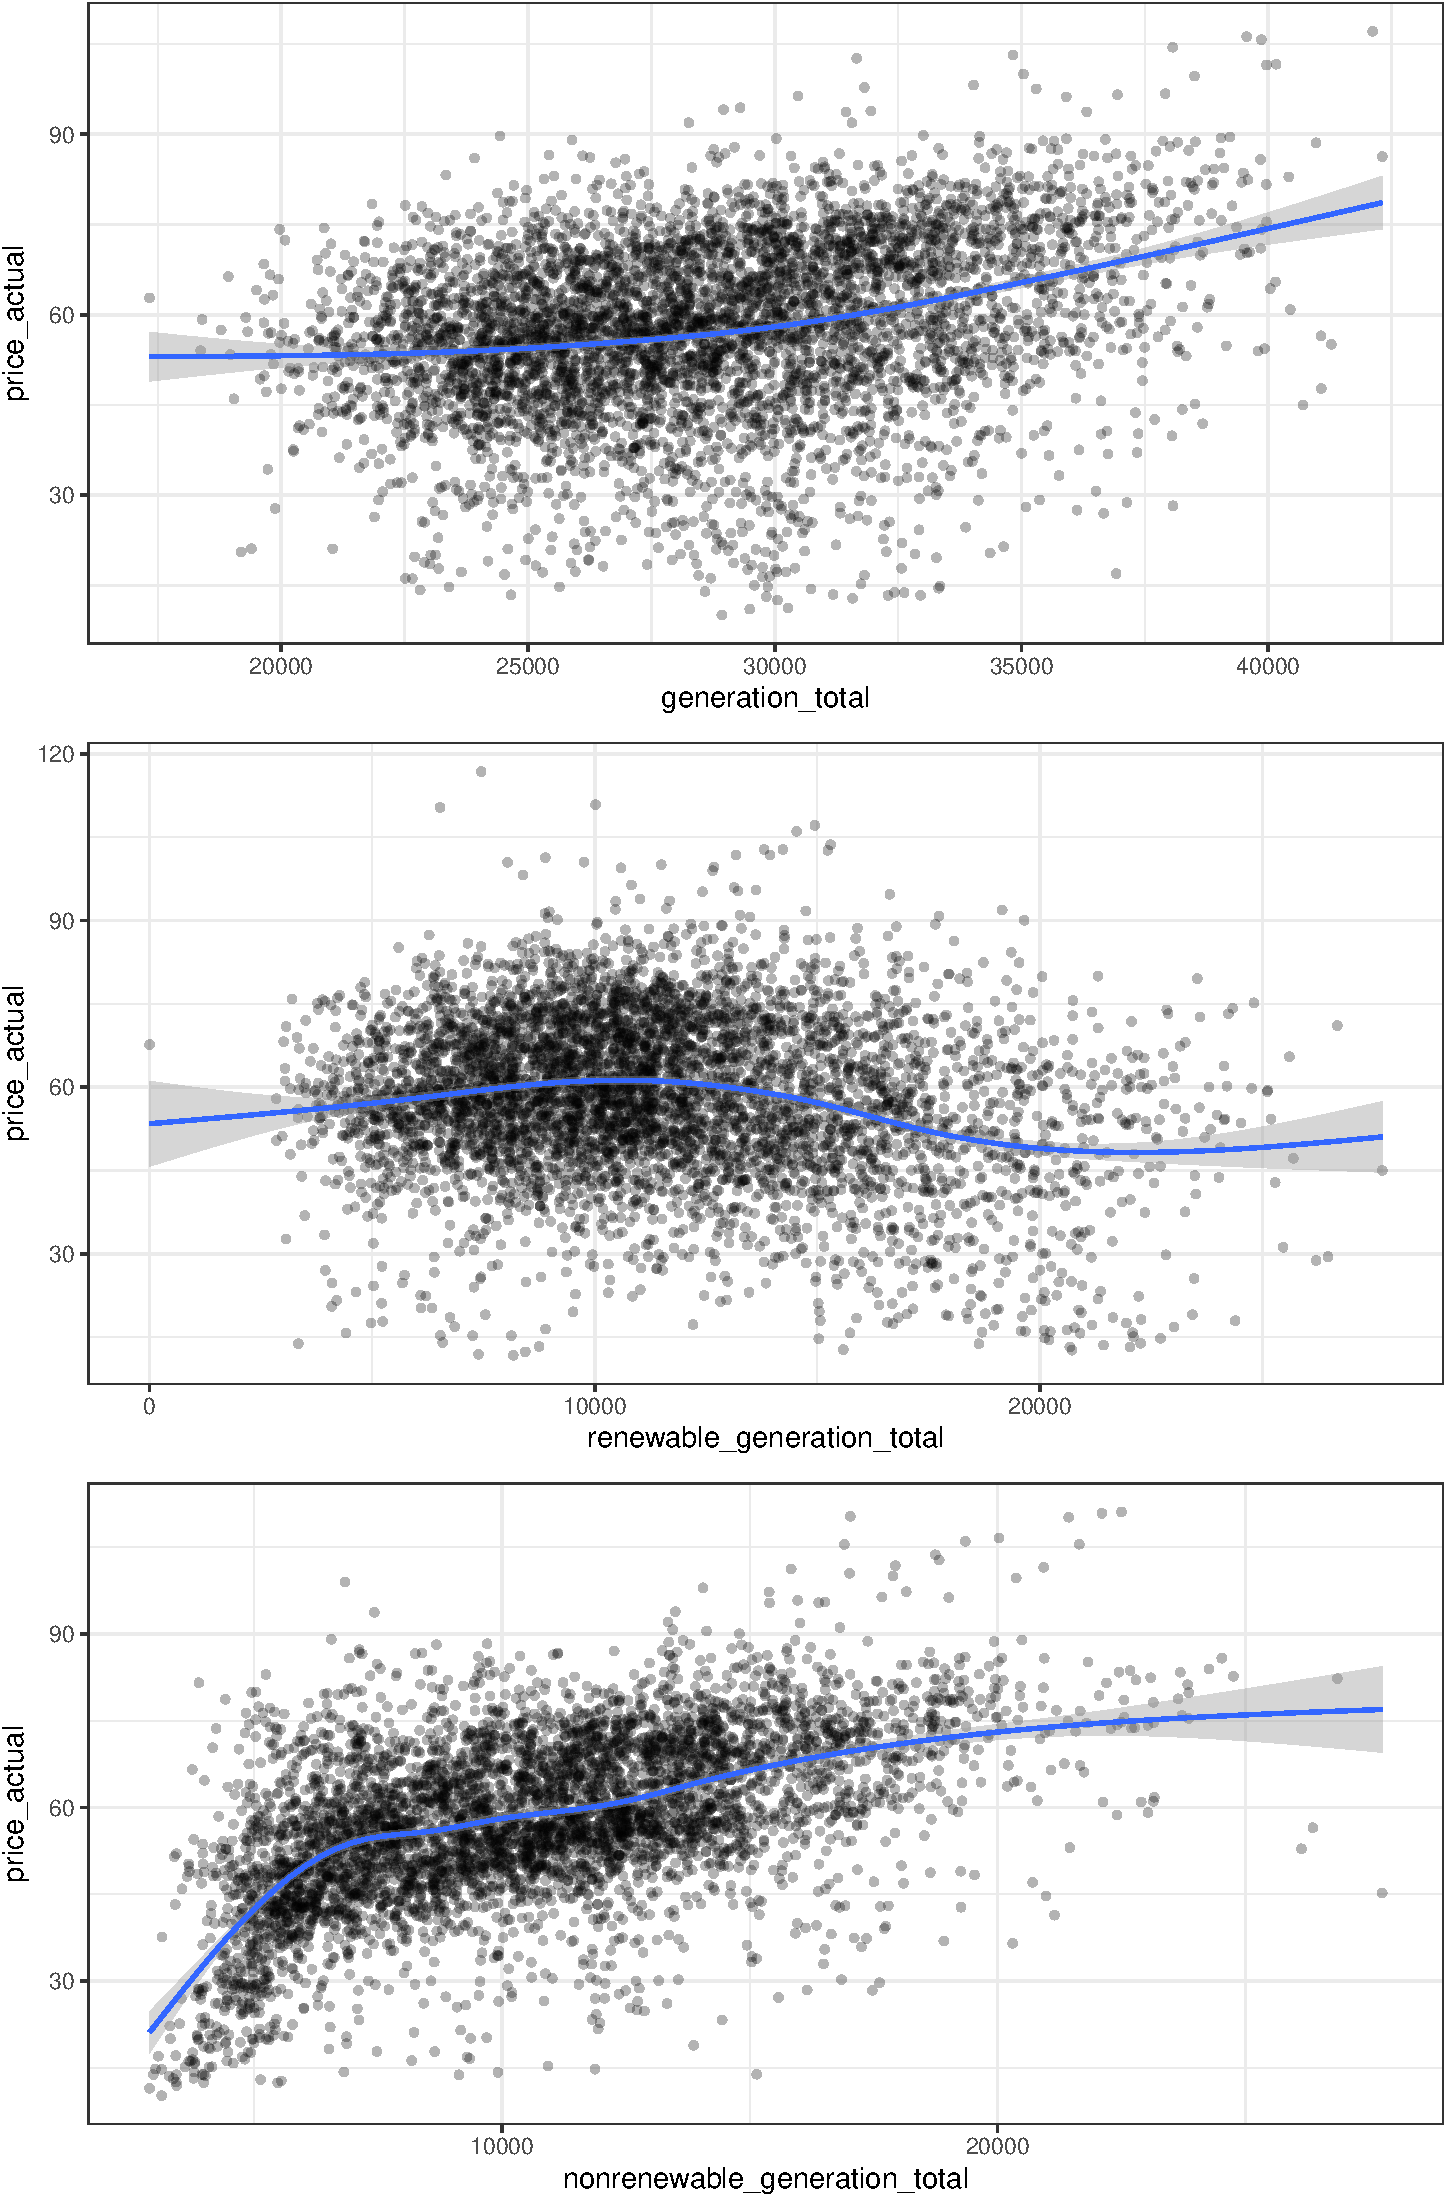
\includegraphics{Analytics_Report_files/figure-pdf/plot167-1.pdf}

We see some interesting relationships in these plots. The
\texttt{generation\_total} and the
\texttt{nonrenewable\_generation\_total} appear to have a positive
relationship, whereas the \texttt{renewable\_generation\_total} doesn't
appear to have a strong positive or negative relationship.

The following plots show the affect of \texttt{total\_load\_actual} and
\texttt{total\_load\_forecast} on the \texttt{price\_actual} response.
We assume that the TSO model to predict prices has access to the load
forecast model, so we will include this predictor in our model
construction.

\begin{Shaded}
\begin{Highlighting}[]
\NormalTok{plot2 }\SpecialCharTok{/}\NormalTok{ plot3}
\end{Highlighting}
\end{Shaded}

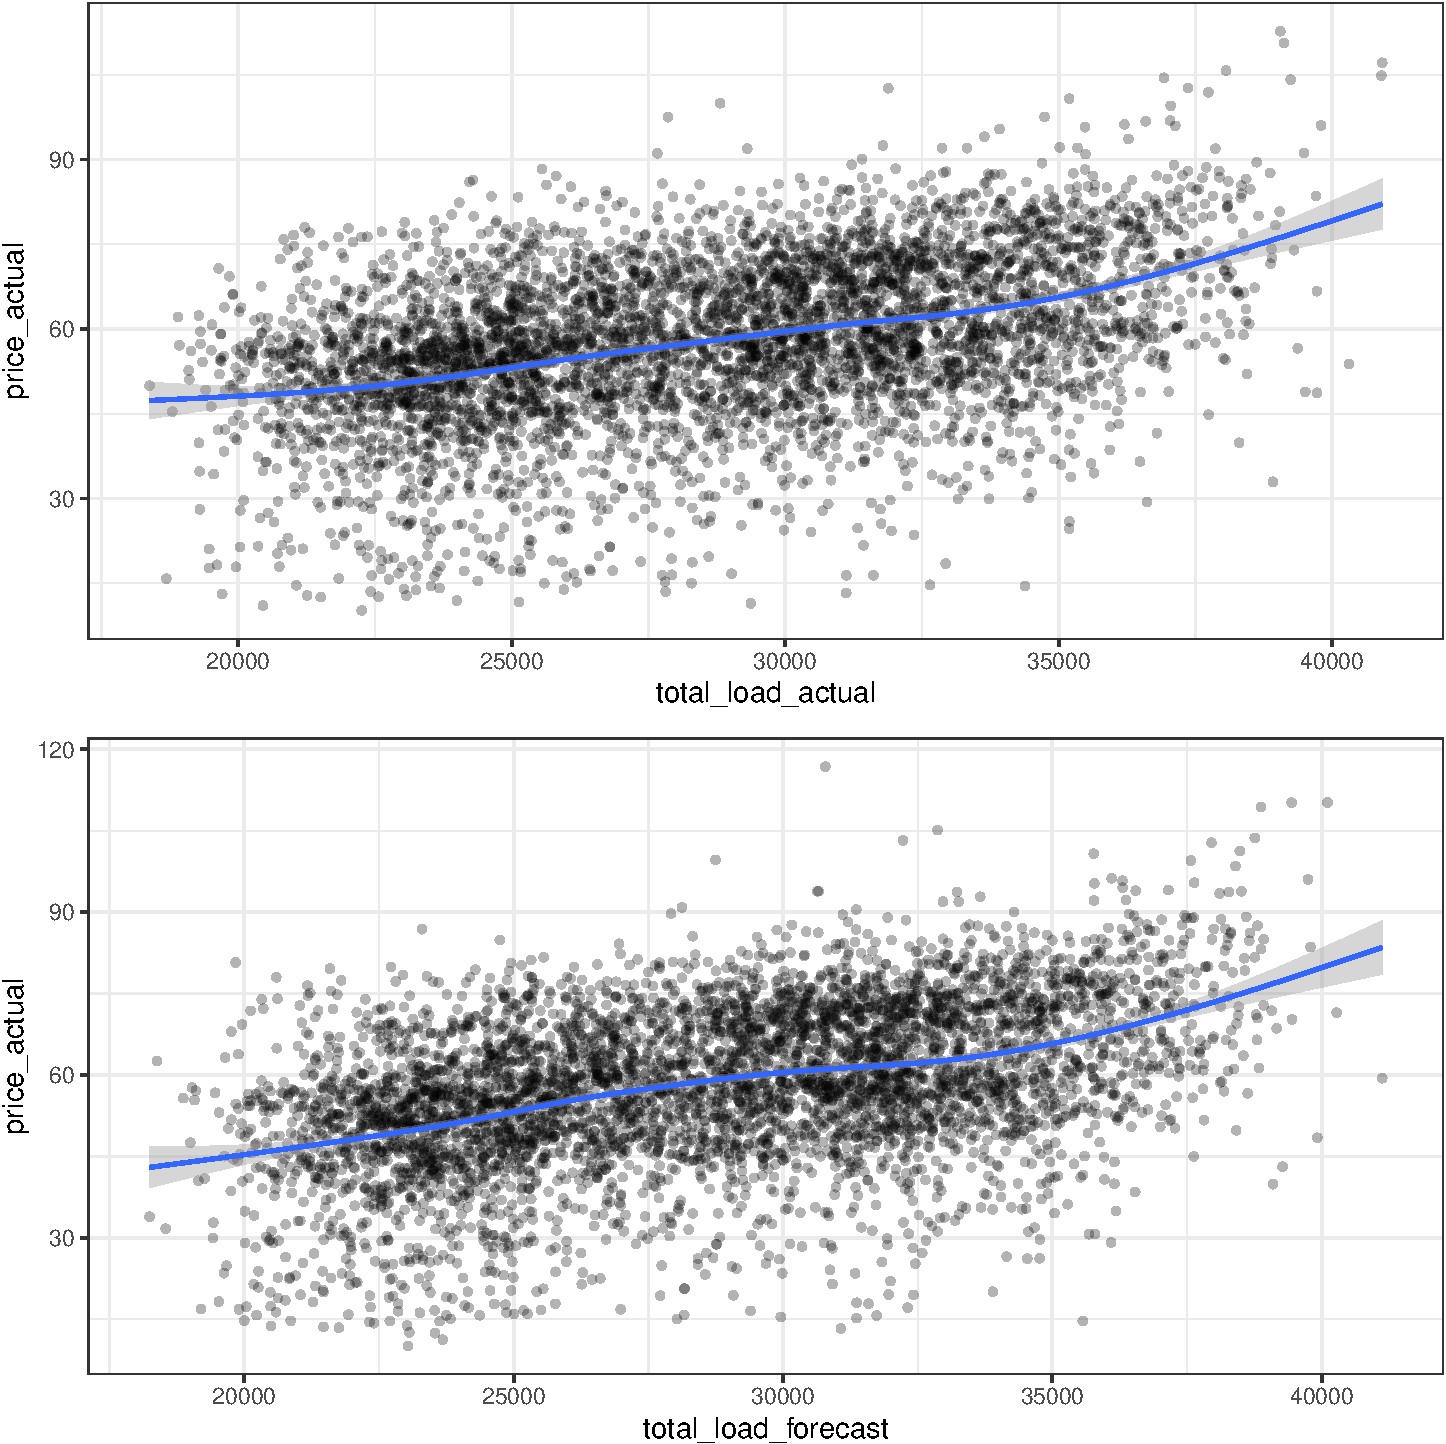
\includegraphics{Analytics_Report_files/figure-pdf/plot23-1.pdf}

Both of these plots seem to show a positive, somewhat linear
relationship.

The following plots are quite interesting, and are built from extracting
data from the \texttt{time} predictor in the dataset. By extracting
\texttt{hour\_of\_day} and \texttt{month\_of\_year}, we can see how
electricity prices change throughout the day and throughout the year.

\begin{Shaded}
\begin{Highlighting}[]
\NormalTok{plot8 }\SpecialCharTok{/}\NormalTok{ plot9}
\end{Highlighting}
\end{Shaded}

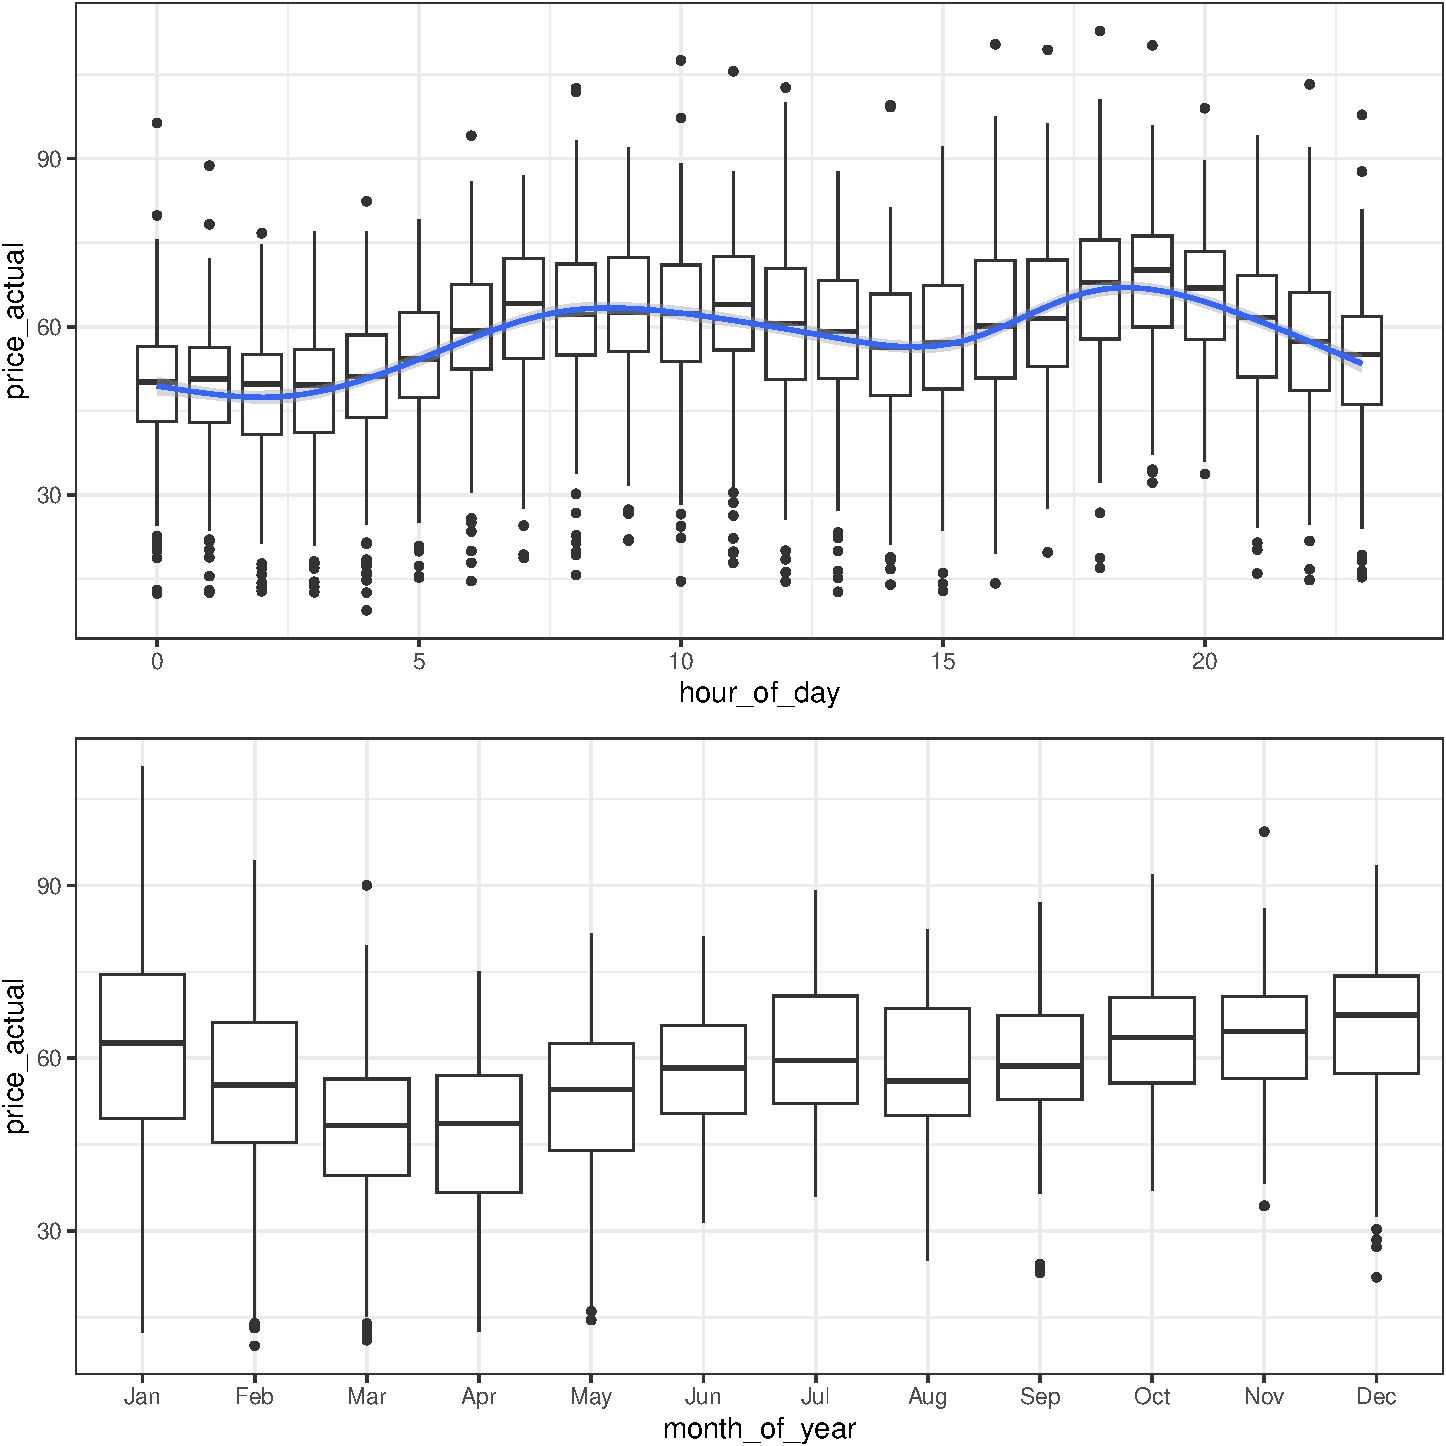
\includegraphics{Analytics_Report_files/figure-pdf/plot89-1.pdf}

These plots show some really clear relationships with curvature. These
strong relationships will certainly improve our model accuracy.

\subsection{Model Construction}\label{model-construction}

We will use cross validation throughout our model construction to
improve our ability to make accurate decisions.

\begin{Shaded}
\begin{Highlighting}[]
\NormalTok{train\_folds }\OtherTok{\textless{}{-}} \FunctionTok{vfold\_cv}\NormalTok{(train, }\AttributeTok{v =} \DecValTok{5}\NormalTok{)}
\end{Highlighting}
\end{Shaded}

\subsubsection{Linear Regression Model}\label{linear-regression-model}

\begin{Shaded}
\begin{Highlighting}[]
\NormalTok{lin\_reg\_spec }\OtherTok{\textless{}{-}} \FunctionTok{linear\_reg}\NormalTok{(}\AttributeTok{penalty =} \FunctionTok{tune}\NormalTok{(), }\AttributeTok{mixture =} \FunctionTok{tune}\NormalTok{()) }\SpecialCharTok{\%\textgreater{}\%}
  \FunctionTok{set\_engine}\NormalTok{(}\StringTok{"glmnet"}\NormalTok{)}

\NormalTok{lin\_reg\_rec }\OtherTok{\textless{}{-}} \FunctionTok{recipe}\NormalTok{(price\_actual }\SpecialCharTok{\textasciitilde{}}\NormalTok{ ., }\AttributeTok{data =}\NormalTok{ predictors) }\SpecialCharTok{\%\textgreater{}\%}
  \FunctionTok{step\_dummy}\NormalTok{(}\FunctionTok{all\_nominal\_predictors}\NormalTok{()) }\SpecialCharTok{|\textgreater{}}
  \FunctionTok{step\_other}\NormalTok{(}\FunctionTok{all\_nominal\_predictors}\NormalTok{()) }\SpecialCharTok{\%\textgreater{}\%}
  \FunctionTok{step\_impute\_median}\NormalTok{(}\FunctionTok{all\_numeric\_predictors}\NormalTok{())}

\NormalTok{lin\_reg\_wf }\OtherTok{\textless{}{-}} \FunctionTok{workflow}\NormalTok{() }\SpecialCharTok{\%\textgreater{}\%}
  \FunctionTok{add\_model}\NormalTok{(lin\_reg\_spec) }\SpecialCharTok{\%\textgreater{}\%}
  \FunctionTok{add\_recipe}\NormalTok{(lin\_reg\_rec)}

\NormalTok{lin\_reg\_grid }\OtherTok{\textless{}{-}} \FunctionTok{grid\_regular}\NormalTok{(}
  \FunctionTok{penalty}\NormalTok{(),}
  \FunctionTok{mixture}\NormalTok{(),}\SpecialCharTok{+}
  \AttributeTok{levels =} \DecValTok{10}
\NormalTok{)}

\NormalTok{n\_cores }\OtherTok{\textless{}{-}}\NormalTok{ parallel}\SpecialCharTok{::}\FunctionTok{detectCores}\NormalTok{()}
\NormalTok{cluster }\OtherTok{\textless{}{-}}\NormalTok{ parallel}\SpecialCharTok{::}\FunctionTok{makeCluster}\NormalTok{(n\_cores }\SpecialCharTok{{-}} \DecValTok{1}\NormalTok{, }\AttributeTok{type =} \StringTok{"PSOCK"}\NormalTok{)}
\NormalTok{doParallel}\SpecialCharTok{::}\FunctionTok{registerDoParallel}\NormalTok{(cluster)}

\NormalTok{tictoc}\SpecialCharTok{::}\FunctionTok{tic}\NormalTok{()}

\NormalTok{lin\_reg\_tune\_results }\OtherTok{\textless{}{-}}\NormalTok{ lin\_reg\_wf }\SpecialCharTok{\%\textgreater{}\%}
  \FunctionTok{tune\_grid}\NormalTok{(}
    \AttributeTok{grid =}\NormalTok{ lin\_reg\_grid,}
    \AttributeTok{resamples =}\NormalTok{ train\_folds}
\NormalTok{  )}

\NormalTok{parallel}\SpecialCharTok{::}\FunctionTok{stopCluster}\NormalTok{(cluster)}

\NormalTok{tictoc}\SpecialCharTok{::}\FunctionTok{toc}\NormalTok{()}
\end{Highlighting}
\end{Shaded}

After using hyper paramater tuning to build a linear regression model,
we look at the 10 best models it built in order of ascending RMSE.

\begin{Shaded}
\begin{Highlighting}[]
\CommentTok{\#save(lin\_reg\_tune\_results, lin\_reg\_wf, file = "lin\_reg\_tune\_results.RData")}
\FunctionTok{load}\NormalTok{(}\StringTok{"lin\_reg\_tune\_results.RData"}\NormalTok{)}

\NormalTok{lin\_reg\_tune\_results }\SpecialCharTok{\%\textgreater{}\%}
  \FunctionTok{show\_best}\NormalTok{(}\AttributeTok{n =} \DecValTok{10}\NormalTok{, }\AttributeTok{metric =} \StringTok{"rmse"}\NormalTok{) }\SpecialCharTok{|\textgreater{}}
  \FunctionTok{kable}\NormalTok{() }\SpecialCharTok{|\textgreater{}}
  \FunctionTok{kable\_styling}\NormalTok{()}
\end{Highlighting}
\end{Shaded}

\begin{longtable*}[t]{rrllrrrl}
\toprule
penalty & mixture & .metric & .estimator & mean & n & std\_err & .config\\
\midrule
0.0059948 & 1.0000000 & rmse & standard & 10.29642 & 5 & 0.0478108 & Preprocessor1\_Model098\\
0.0059948 & 0.8888889 & rmse & standard & 10.29647 & 5 & 0.0478723 & Preprocessor1\_Model088\\
0.0059948 & 0.7777778 & rmse & standard & 10.29658 & 5 & 0.0479133 & Preprocessor1\_Model078\\
0.0000000 & 0.1111111 & rmse & standard & 10.29662 & 5 & 0.0481989 & Preprocessor1\_Model011\\
0.0000000 & 0.1111111 & rmse & standard & 10.29662 & 5 & 0.0481989 & Preprocessor1\_Model012\\
\addlinespace
0.0000000 & 0.1111111 & rmse & standard & 10.29662 & 5 & 0.0481989 & Preprocessor1\_Model013\\
0.0000002 & 0.1111111 & rmse & standard & 10.29662 & 5 & 0.0481989 & Preprocessor1\_Model014\\
0.0000028 & 0.1111111 & rmse & standard & 10.29662 & 5 & 0.0481989 & Preprocessor1\_Model015\\
0.0000359 & 0.1111111 & rmse & standard & 10.29662 & 5 & 0.0481989 & Preprocessor1\_Model016\\
0.0004642 & 0.1111111 & rmse & standard & 10.29662 & 5 & 0.0481989 & Preprocessor1\_Model017\\
\bottomrule
\end{longtable*}

\begin{Shaded}
\begin{Highlighting}[]
\NormalTok{best\_lin\_reg }\OtherTok{\textless{}{-}}\NormalTok{ lin\_reg\_tune\_results }\SpecialCharTok{\%\textgreater{}\%}
  \FunctionTok{select\_best}\NormalTok{(}\AttributeTok{metric =} \StringTok{"rmse"}\NormalTok{)}

\NormalTok{lin\_reg\_wf\_final }\OtherTok{\textless{}{-}}\NormalTok{ lin\_reg\_wf }\SpecialCharTok{\%\textgreater{}\%}
  \FunctionTok{finalize\_workflow}\NormalTok{(best\_lin\_reg)}

\NormalTok{lin\_reg\_fit }\OtherTok{\textless{}{-}}\NormalTok{ lin\_reg\_wf\_final }\SpecialCharTok{\%\textgreater{}\%}
  \FunctionTok{fit}\NormalTok{(train)}
\end{Highlighting}
\end{Shaded}

We fit the best model to our training data, and calculate the RMSE.

\begin{Shaded}
\begin{Highlighting}[]
\CommentTok{\#save(lin\_reg\_fit, file = "lin\_reg\_fit.RData")}
\FunctionTok{load}\NormalTok{(}\StringTok{"lin\_reg\_fit.RData"}\NormalTok{)}

\NormalTok{lin\_reg\_predictions\_train }\OtherTok{\textless{}{-}}\NormalTok{ lin\_reg\_fit }\SpecialCharTok{|\textgreater{}}
  \FunctionTok{augment}\NormalTok{(train) }\SpecialCharTok{|\textgreater{}}
  \FunctionTok{select}\NormalTok{(.pred, price\_actual) }\SpecialCharTok{|\textgreater{}}
  \FunctionTok{rename}\NormalTok{(}\AttributeTok{.pred\_lin\_reg\_train =}\NormalTok{ .pred)}

\NormalTok{lin\_reg\_predictions\_train }\SpecialCharTok{|\textgreater{}}
  \FunctionTok{rmse}\NormalTok{(.pred\_lin\_reg\_train, price\_actual) }\SpecialCharTok{|\textgreater{}}
  \FunctionTok{kable}\NormalTok{() }\SpecialCharTok{|\textgreater{}}
  \FunctionTok{kable\_styling}\NormalTok{()}
\end{Highlighting}
\end{Shaded}

\begin{longtable*}[t]{llr}
\toprule
.metric & .estimator & .estimate\\
\midrule
rmse & standard & 10.28414\\
\bottomrule
\end{longtable*}

On the training data, we see that this linear regression model has an
RMSE of 10.28, which is already outperforming the TSO RMSE of 13.25.

Let's make predictions on the \texttt{validation} data set.

\begin{Shaded}
\begin{Highlighting}[]
\NormalTok{lin\_reg\_predictions\_validation }\OtherTok{\textless{}{-}}\NormalTok{ lin\_reg\_fit }\SpecialCharTok{|\textgreater{}}
  \FunctionTok{augment}\NormalTok{(validation) }\SpecialCharTok{|\textgreater{}}
  \FunctionTok{select}\NormalTok{(.pred, price\_actual) }\SpecialCharTok{|\textgreater{}}
  \FunctionTok{rename}\NormalTok{(}\AttributeTok{.pred\_lin\_reg\_validation =}\NormalTok{ .pred)}

\NormalTok{lin\_reg\_predictions\_validation }\SpecialCharTok{|\textgreater{}}
  \FunctionTok{rmse}\NormalTok{(.pred\_lin\_reg\_validation, price\_actual) }\SpecialCharTok{|\textgreater{}}
  \FunctionTok{kable}\NormalTok{() }\SpecialCharTok{|\textgreater{}}
  \FunctionTok{kable\_styling}\NormalTok{()}
\end{Highlighting}
\end{Shaded}

\begin{longtable*}[t]{llr}
\toprule
.metric & .estimator & .estimate\\
\midrule
rmse & standard & 10.21945\\
\bottomrule
\end{longtable*}

We see that our RMSE on the \texttt{validation} data is 10.22, which
interestingly is better than the training data.

Let's plot our predictions against the true values.

\begin{Shaded}
\begin{Highlighting}[]
\NormalTok{xVals1 }\OtherTok{\textless{}{-}} \FunctionTok{runif}\NormalTok{(}\DecValTok{26298}\NormalTok{, }\AttributeTok{min =} \DecValTok{0}\NormalTok{, }\AttributeTok{max =} \DecValTok{120}\NormalTok{)}
\NormalTok{yVals1 }\OtherTok{\textless{}{-}}\NormalTok{ xVals1}
\CommentTok{\#linedata \textless{}{-} tibble(x = xVals, y = yVals)}

\NormalTok{xVals2 }\OtherTok{\textless{}{-}} \FunctionTok{runif}\NormalTok{(}\DecValTok{4383}\NormalTok{, }\AttributeTok{min =} \DecValTok{0}\NormalTok{, }\AttributeTok{max =} \DecValTok{120}\NormalTok{)}
\NormalTok{yVals2 }\OtherTok{\textless{}{-}}\NormalTok{ xVals2}

\NormalTok{lin\_reg\_plot\_train }\OtherTok{\textless{}{-}}\NormalTok{ lin\_reg\_predictions\_train }\SpecialCharTok{|\textgreater{}}
  \FunctionTok{mutate}\NormalTok{(xVals1, yVals1) }\SpecialCharTok{|\textgreater{}}
  \FunctionTok{ggplot}\NormalTok{() }\SpecialCharTok{+}
  \FunctionTok{geom\_point}\NormalTok{(}\FunctionTok{aes}\NormalTok{(}\AttributeTok{x =}\NormalTok{ .pred\_lin\_reg\_train, }\AttributeTok{y =}\NormalTok{ price\_actual)) }\SpecialCharTok{+}
  \FunctionTok{geom\_point}\NormalTok{(}\FunctionTok{aes}\NormalTok{(}\AttributeTok{x =}\NormalTok{ xVals1, }\AttributeTok{y =}\NormalTok{ yVals1), }\AttributeTok{color =} \StringTok{\textquotesingle{}blue\textquotesingle{}}\NormalTok{, }\AttributeTok{size =} \FloatTok{0.5}\NormalTok{)}

\NormalTok{lin\_reg\_plot\_validation }\OtherTok{\textless{}{-}}\NormalTok{ lin\_reg\_predictions\_validation }\SpecialCharTok{|\textgreater{}}
  \FunctionTok{mutate}\NormalTok{(xVals2, yVals2) }\SpecialCharTok{|\textgreater{}}
  \FunctionTok{ggplot}\NormalTok{() }\SpecialCharTok{+}
  \FunctionTok{geom\_point}\NormalTok{(}\FunctionTok{aes}\NormalTok{(}\AttributeTok{x =}\NormalTok{ .pred\_lin\_reg\_validation, }\AttributeTok{y =}\NormalTok{ price\_actual)) }\SpecialCharTok{+}
  \FunctionTok{geom\_point}\NormalTok{(}\FunctionTok{aes}\NormalTok{(}\AttributeTok{x =}\NormalTok{ xVals2, }\AttributeTok{y =}\NormalTok{ yVals2), }\AttributeTok{color =} \StringTok{\textquotesingle{}blue\textquotesingle{}}\NormalTok{, }\AttributeTok{size =} \FloatTok{0.5}\NormalTok{)}

\NormalTok{lin\_reg\_plot\_train }\SpecialCharTok{+}\NormalTok{ lin\_reg\_plot\_validation}
\end{Highlighting}
\end{Shaded}

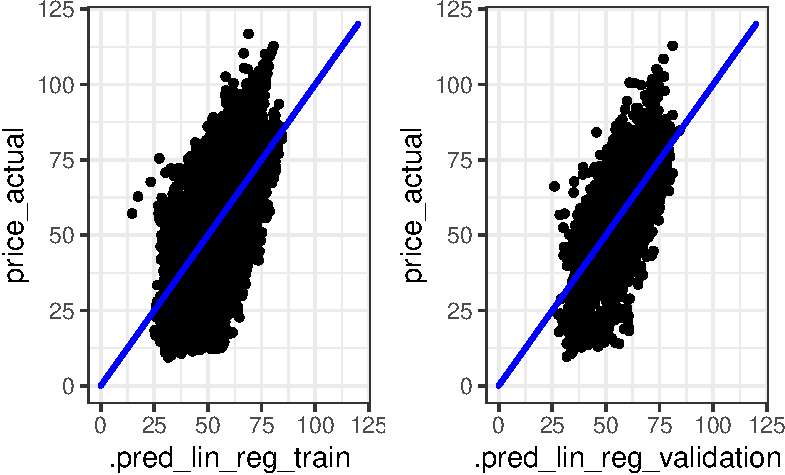
\includegraphics{Analytics_Report_files/figure-pdf/plotLinReg-1.pdf}

From these plots, we can see that this model is outperforming the TSO
model, but still can be improved.

\subsubsection{Random Forest Model}\label{random-forest-model}

\begin{Shaded}
\begin{Highlighting}[]
\NormalTok{rf\_spec }\OtherTok{\textless{}{-}} \FunctionTok{rand\_forest}\NormalTok{(}\AttributeTok{mtry =} \FunctionTok{tune}\NormalTok{(), }\AttributeTok{trees =} \FunctionTok{tune}\NormalTok{()) }\SpecialCharTok{\%\textgreater{}\%}
  \FunctionTok{set\_engine}\NormalTok{(}\StringTok{"ranger"}\NormalTok{) }\SpecialCharTok{\%\textgreater{}\%}
  \FunctionTok{set\_mode}\NormalTok{(}\StringTok{"regression"}\NormalTok{)}

\NormalTok{rf\_rec }\OtherTok{\textless{}{-}} \FunctionTok{recipe}\NormalTok{(price\_actual }\SpecialCharTok{\textasciitilde{}}\NormalTok{ ., }\AttributeTok{data =}\NormalTok{ predictors) }\SpecialCharTok{\%\textgreater{}\%}
  \FunctionTok{step\_dummy}\NormalTok{(}\FunctionTok{all\_nominal\_predictors}\NormalTok{()) }\SpecialCharTok{|\textgreater{}}
  \FunctionTok{step\_other}\NormalTok{(}\FunctionTok{all\_nominal\_predictors}\NormalTok{()) }\SpecialCharTok{\%\textgreater{}\%}
  \FunctionTok{step\_impute\_median}\NormalTok{(}\FunctionTok{all\_numeric\_predictors}\NormalTok{())}

\NormalTok{rf\_wf }\OtherTok{\textless{}{-}} \FunctionTok{workflow}\NormalTok{() }\SpecialCharTok{\%\textgreater{}\%}
  \FunctionTok{add\_model}\NormalTok{(rf\_spec) }\SpecialCharTok{\%\textgreater{}\%}
  \FunctionTok{add\_recipe}\NormalTok{(rf\_rec)}

\NormalTok{rf\_grid }\OtherTok{\textless{}{-}} \FunctionTok{grid\_regular}\NormalTok{(}
  \FunctionTok{mtry}\NormalTok{(}\AttributeTok{range =} \FunctionTok{c}\NormalTok{(}\DecValTok{1}\NormalTok{, }\DecValTok{10}\NormalTok{)),}
  \FunctionTok{trees}\NormalTok{(),}
  \AttributeTok{levels =} \DecValTok{5}
\NormalTok{)}

\NormalTok{n\_cores }\OtherTok{\textless{}{-}}\NormalTok{ parallel}\SpecialCharTok{::}\FunctionTok{detectCores}\NormalTok{()}
\NormalTok{cluster }\OtherTok{\textless{}{-}}\NormalTok{ parallel}\SpecialCharTok{::}\FunctionTok{makeCluster}\NormalTok{(n\_cores }\SpecialCharTok{{-}} \DecValTok{1}\NormalTok{, }\AttributeTok{type =} \StringTok{"PSOCK"}\NormalTok{)}
\NormalTok{doParallel}\SpecialCharTok{::}\FunctionTok{registerDoParallel}\NormalTok{(cluster)}

\NormalTok{tictoc}\SpecialCharTok{::}\FunctionTok{tic}\NormalTok{()}

\NormalTok{rf\_tune\_results }\OtherTok{\textless{}{-}}\NormalTok{ rf\_wf }\SpecialCharTok{\%\textgreater{}\%}
  \FunctionTok{tune\_grid}\NormalTok{(}
    \AttributeTok{grid =}\NormalTok{ rf\_grid,}
    \AttributeTok{resamples =}\NormalTok{ train\_folds}
\NormalTok{  )}

\NormalTok{parallel}\SpecialCharTok{::}\FunctionTok{stopCluster}\NormalTok{(cluster)}

\NormalTok{tictoc}\SpecialCharTok{::}\FunctionTok{toc}\NormalTok{()}
\end{Highlighting}
\end{Shaded}

After using hyperparamater tuning to build a random forest model, we
show the best 10 models in order of ascending RMSE.

\begin{Shaded}
\begin{Highlighting}[]
\CommentTok{\#save(rf\_tune\_results, rf\_wf, file = "rf\_tune\_results.RData")}
\FunctionTok{load}\NormalTok{(}\StringTok{"rf\_tune\_results.RData"}\NormalTok{)}

\NormalTok{rf\_tune\_results }\SpecialCharTok{\%\textgreater{}\%}
  \FunctionTok{show\_best}\NormalTok{(}\AttributeTok{n =} \DecValTok{10}\NormalTok{, }\AttributeTok{metric =} \StringTok{"rmse"}\NormalTok{) }\SpecialCharTok{|\textgreater{}}
  \FunctionTok{kable}\NormalTok{() }\SpecialCharTok{|\textgreater{}}
  \FunctionTok{kable\_styling}\NormalTok{()}
\end{Highlighting}
\end{Shaded}

\begin{longtable*}[t]{rrllrrrl}
\toprule
mtry & trees & .metric & .estimator & mean & n & std\_err & .config\\
\midrule
10 & 2000 & rmse & standard & 4.570574 & 5 & 0.0472913 & Preprocessor1\_Model25\\
10 & 1500 & rmse & standard & 4.571607 & 5 & 0.0477593 & Preprocessor1\_Model20\\
10 & 1000 & rmse & standard & 4.572664 & 5 & 0.0472862 & Preprocessor1\_Model15\\
10 & 500 & rmse & standard & 4.588664 & 5 & 0.0468897 & Preprocessor1\_Model10\\
7 & 2000 & rmse & standard & 4.633177 & 5 & 0.0488629 & Preprocessor1\_Model24\\
\addlinespace
7 & 1500 & rmse & standard & 4.635829 & 5 & 0.0483290 & Preprocessor1\_Model19\\
7 & 1000 & rmse & standard & 4.638231 & 5 & 0.0453621 & Preprocessor1\_Model14\\
7 & 500 & rmse & standard & 4.641607 & 5 & 0.0442504 & Preprocessor1\_Model09\\
5 & 1500 & rmse & standard & 4.782919 & 5 & 0.0448245 & Preprocessor1\_Model18\\
5 & 2000 & rmse & standard & 4.783133 & 5 & 0.0454290 & Preprocessor1\_Model23\\
\bottomrule
\end{longtable*}

\begin{Shaded}
\begin{Highlighting}[]
\NormalTok{best\_rf }\OtherTok{\textless{}{-}}\NormalTok{ rf\_tune\_results }\SpecialCharTok{\%\textgreater{}\%}
  \FunctionTok{select\_best}\NormalTok{(}\AttributeTok{metric =} \StringTok{"rmse"}\NormalTok{)}

\NormalTok{rf\_wf\_final }\OtherTok{\textless{}{-}}\NormalTok{ rf\_wf }\SpecialCharTok{\%\textgreater{}\%}
  \FunctionTok{finalize\_workflow}\NormalTok{(best\_rf)}

\NormalTok{rf\_fit }\OtherTok{\textless{}{-}}\NormalTok{ rf\_wf\_final }\SpecialCharTok{\%\textgreater{}\%}
  \FunctionTok{fit}\NormalTok{(train)}
\end{Highlighting}
\end{Shaded}

We fit our best model to the training data, and calculate the RMSE.

\begin{Shaded}
\begin{Highlighting}[]
\CommentTok{\#save(rf\_fit, file = "rf\_fit.RData")}
\FunctionTok{load}\NormalTok{(}\StringTok{"rf\_fit.RData"}\NormalTok{)}

\NormalTok{rf\_predictions\_train }\OtherTok{\textless{}{-}}\NormalTok{ rf\_fit }\SpecialCharTok{|\textgreater{}}
  \FunctionTok{augment}\NormalTok{(train) }\SpecialCharTok{|\textgreater{}}
  \FunctionTok{select}\NormalTok{(.pred, price\_actual) }\SpecialCharTok{|\textgreater{}}
  \FunctionTok{rename}\NormalTok{(}\AttributeTok{.pred\_rf\_train =}\NormalTok{ .pred)}

\NormalTok{rf\_predictions\_train }\SpecialCharTok{|\textgreater{}}
  \FunctionTok{rmse}\NormalTok{(.pred\_rf\_train, price\_actual) }\SpecialCharTok{|\textgreater{}}
  \FunctionTok{kable}\NormalTok{() }\SpecialCharTok{|\textgreater{}}
  \FunctionTok{kable\_styling}\NormalTok{()}
\end{Highlighting}
\end{Shaded}

\begin{longtable*}[t]{llr}
\toprule
.metric & .estimator & .estimate\\
\midrule
rmse & standard & 1.772513\\
\bottomrule
\end{longtable*}

On the training data, we see a RMSE of 1.77! This is quite a bit better
than the linear regression model and the TSO model.

Let's make predictions for our \texttt{validation} dataset.

\begin{Shaded}
\begin{Highlighting}[]
\NormalTok{rf\_predictions\_validation }\OtherTok{\textless{}{-}}\NormalTok{ rf\_fit }\SpecialCharTok{|\textgreater{}}
  \FunctionTok{augment}\NormalTok{(validation) }\SpecialCharTok{|\textgreater{}}
  \FunctionTok{select}\NormalTok{(.pred, price\_actual) }\SpecialCharTok{|\textgreater{}}
  \FunctionTok{rename}\NormalTok{(}\AttributeTok{.pred\_rf\_validation =}\NormalTok{ .pred)}

\NormalTok{rf\_predictions\_validation }\SpecialCharTok{|\textgreater{}}
  \FunctionTok{rmse}\NormalTok{(.pred\_rf\_validation, price\_actual) }\SpecialCharTok{|\textgreater{}}
  \FunctionTok{kable}\NormalTok{() }\SpecialCharTok{|\textgreater{}}
  \FunctionTok{kable\_styling}\NormalTok{()}
\end{Highlighting}
\end{Shaded}

\begin{longtable*}[t]{llr}
\toprule
.metric & .estimator & .estimate\\
\midrule
rmse & standard & 4.118898\\
\bottomrule
\end{longtable*}

The RMSE for our \texttt{validation} dataset was 4.12, which is worse
than the RMSE on the training data, however it is still significantly
better than the RMSE of the linear regression and the TSO models.

Let's plot our predictions compared to the true day ahead prices.

\begin{Shaded}
\begin{Highlighting}[]
\NormalTok{xVals1 }\OtherTok{\textless{}{-}} \FunctionTok{runif}\NormalTok{(}\DecValTok{26298}\NormalTok{, }\AttributeTok{min =} \DecValTok{0}\NormalTok{, }\AttributeTok{max =} \DecValTok{120}\NormalTok{)}
\NormalTok{yVals1 }\OtherTok{\textless{}{-}}\NormalTok{ xVals1}
\CommentTok{\#linedata \textless{}{-} tibble(x = xVals, y = yVals)}

\NormalTok{xVals2 }\OtherTok{\textless{}{-}} \FunctionTok{runif}\NormalTok{(}\DecValTok{4383}\NormalTok{, }\AttributeTok{min =} \DecValTok{0}\NormalTok{, }\AttributeTok{max =} \DecValTok{120}\NormalTok{)}
\NormalTok{yVals2 }\OtherTok{\textless{}{-}}\NormalTok{ xVals2}

\NormalTok{rf\_plot\_train }\OtherTok{\textless{}{-}}\NormalTok{ rf\_predictions\_train }\SpecialCharTok{|\textgreater{}}
  \FunctionTok{mutate}\NormalTok{(xVals1, yVals1) }\SpecialCharTok{|\textgreater{}}
  \FunctionTok{ggplot}\NormalTok{() }\SpecialCharTok{+}
  \FunctionTok{geom\_point}\NormalTok{(}\FunctionTok{aes}\NormalTok{(}\AttributeTok{x =}\NormalTok{ .pred\_rf\_train, }\AttributeTok{y =}\NormalTok{ price\_actual)) }\SpecialCharTok{+}
  \FunctionTok{geom\_point}\NormalTok{(}\FunctionTok{aes}\NormalTok{(}\AttributeTok{x =}\NormalTok{ xVals1, }\AttributeTok{y =}\NormalTok{ yVals1), }\AttributeTok{color =} \StringTok{\textquotesingle{}blue\textquotesingle{}}\NormalTok{, }\AttributeTok{size =} \FloatTok{0.5}\NormalTok{)}

\NormalTok{rf\_plot\_validation }\OtherTok{\textless{}{-}}\NormalTok{ rf\_predictions\_validation }\SpecialCharTok{|\textgreater{}}
  \FunctionTok{mutate}\NormalTok{(xVals2, yVals2) }\SpecialCharTok{|\textgreater{}}
  \FunctionTok{ggplot}\NormalTok{() }\SpecialCharTok{+}
  \FunctionTok{geom\_point}\NormalTok{(}\FunctionTok{aes}\NormalTok{(}\AttributeTok{x =}\NormalTok{ .pred\_rf\_validation, }\AttributeTok{y =}\NormalTok{ price\_actual)) }\SpecialCharTok{+}
  \FunctionTok{geom\_point}\NormalTok{(}\FunctionTok{aes}\NormalTok{(}\AttributeTok{x =}\NormalTok{ xVals2, }\AttributeTok{y =}\NormalTok{ yVals2), }\AttributeTok{color =} \StringTok{\textquotesingle{}blue\textquotesingle{}}\NormalTok{, }\AttributeTok{size =} \FloatTok{0.5}\NormalTok{)}

\NormalTok{rf\_plot\_train }\SpecialCharTok{+}\NormalTok{ rf\_plot\_validation}
\end{Highlighting}
\end{Shaded}

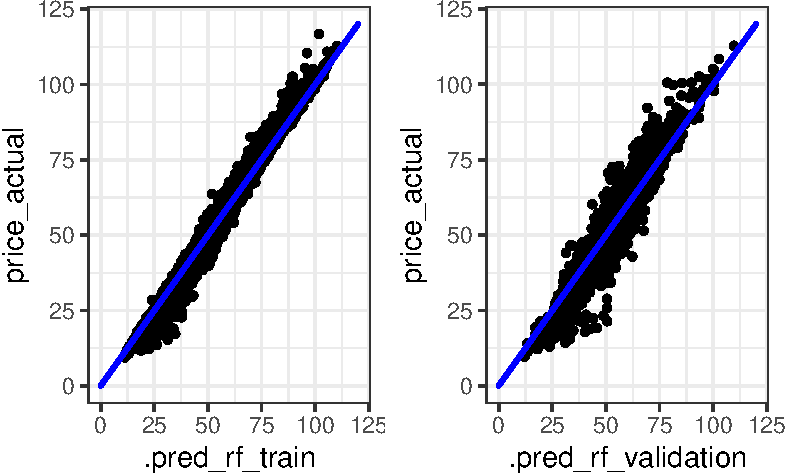
\includegraphics{Analytics_Report_files/figure-pdf/plotRf-1.pdf}

We see that the predictions from the random forest model are
significantly better, and are getting closer and closer to the line
\(y = x\), the ideal model. We will see if we can improve upon this in
our last model class, extreme gradient boosting.

\subsubsection{Extreme Gradient Boosting
Model}\label{extreme-gradient-boosting-model}

\begin{Shaded}
\begin{Highlighting}[]
\NormalTok{xgb\_spec }\OtherTok{\textless{}{-}} \FunctionTok{boost\_tree}\NormalTok{(}\AttributeTok{mtry =} \FunctionTok{tune}\NormalTok{(), }\AttributeTok{trees =} \FunctionTok{tune}\NormalTok{(), }\AttributeTok{learn\_rate =} \FunctionTok{tune}\NormalTok{()) }\SpecialCharTok{\%\textgreater{}\%}
  \FunctionTok{set\_engine}\NormalTok{(}\StringTok{"xgboost"}\NormalTok{) }\SpecialCharTok{\%\textgreater{}\%}
  \FunctionTok{set\_mode}\NormalTok{(}\StringTok{"regression"}\NormalTok{)}

\NormalTok{xgb\_rec }\OtherTok{\textless{}{-}} \FunctionTok{recipe}\NormalTok{(price\_actual }\SpecialCharTok{\textasciitilde{}}\NormalTok{ ., }\AttributeTok{data =}\NormalTok{ predictors) }\SpecialCharTok{\%\textgreater{}\%}
  \FunctionTok{step\_dummy}\NormalTok{(}\FunctionTok{all\_nominal\_predictors}\NormalTok{()) }\SpecialCharTok{|\textgreater{}}
  \FunctionTok{step\_other}\NormalTok{(}\FunctionTok{all\_nominal\_predictors}\NormalTok{()) }\SpecialCharTok{\%\textgreater{}\%}
  \FunctionTok{step\_impute\_median}\NormalTok{(}\FunctionTok{all\_numeric\_predictors}\NormalTok{())}

\NormalTok{xgb\_wf }\OtherTok{\textless{}{-}} \FunctionTok{workflow}\NormalTok{() }\SpecialCharTok{\%\textgreater{}\%}
  \FunctionTok{add\_model}\NormalTok{(xgb\_spec) }\SpecialCharTok{\%\textgreater{}\%}
  \FunctionTok{add\_recipe}\NormalTok{(xgb\_rec)}

\NormalTok{xgb\_grid }\OtherTok{\textless{}{-}} \FunctionTok{grid\_regular}\NormalTok{(}
  \FunctionTok{mtry}\NormalTok{(}\AttributeTok{range =} \FunctionTok{c}\NormalTok{(}\DecValTok{1}\NormalTok{, }\DecValTok{10}\NormalTok{)),}
  \FunctionTok{trees}\NormalTok{(),}
  \FunctionTok{learn\_rate}\NormalTok{(),}
  \AttributeTok{levels =} \DecValTok{5}
\NormalTok{)}

\NormalTok{n\_cores }\OtherTok{\textless{}{-}}\NormalTok{ parallel}\SpecialCharTok{::}\FunctionTok{detectCores}\NormalTok{()}
\NormalTok{cluster }\OtherTok{\textless{}{-}}\NormalTok{ parallel}\SpecialCharTok{::}\FunctionTok{makeCluster}\NormalTok{(n\_cores }\SpecialCharTok{{-}} \DecValTok{1}\NormalTok{, }\AttributeTok{type =} \StringTok{"PSOCK"}\NormalTok{)}
\NormalTok{doParallel}\SpecialCharTok{::}\FunctionTok{registerDoParallel}\NormalTok{(cluster)}

\NormalTok{tictoc}\SpecialCharTok{::}\FunctionTok{tic}\NormalTok{()}

\NormalTok{xgb\_tune\_results }\OtherTok{\textless{}{-}}\NormalTok{ xgb\_wf }\SpecialCharTok{\%\textgreater{}\%}
  \FunctionTok{tune\_grid}\NormalTok{(}
    \AttributeTok{grid =}\NormalTok{ xgb\_grid,}
    \AttributeTok{resamples =}\NormalTok{ train\_folds}
\NormalTok{  )}

\NormalTok{parallel}\SpecialCharTok{::}\FunctionTok{stopCluster}\NormalTok{(cluster)}

\NormalTok{tictoc}\SpecialCharTok{::}\FunctionTok{toc}\NormalTok{()}
\end{Highlighting}
\end{Shaded}

After using hyperparamater tuning to build an extreme gradient boosting
model, we show the best 10 models in order of ascending RMSE.

\begin{Shaded}
\begin{Highlighting}[]
\CommentTok{\#save(xgb\_tune\_results, xgb\_wf, file = "xgb\_tune\_results.RData")}
\FunctionTok{load}\NormalTok{(}\StringTok{"xgb\_tune\_results.RData"}\NormalTok{)}

\NormalTok{xgb\_tune\_results }\SpecialCharTok{\%\textgreater{}\%}
  \FunctionTok{show\_best}\NormalTok{(}\AttributeTok{n =} \DecValTok{10}\NormalTok{, }\AttributeTok{metric =} \StringTok{"rmse"}\NormalTok{) }\SpecialCharTok{|\textgreater{}}
  \FunctionTok{kable}\NormalTok{() }\SpecialCharTok{|\textgreater{}}
  \FunctionTok{kable\_styling}\NormalTok{()}
\end{Highlighting}
\end{Shaded}

\begin{longtable*}[t]{rrrllrrrl}
\toprule
mtry & trees & learn\_rate & .metric & .estimator & mean & n & std\_err & .config\\
\midrule
7 & 2000 & 0.1 & rmse & standard & 3.790247 & 5 & 0.0350662 & Preprocessor1\_Model100\\
5 & 2000 & 0.1 & rmse & standard & 3.795045 & 5 & 0.0429371 & Preprocessor1\_Model075\\
10 & 2000 & 0.1 & rmse & standard & 3.803137 & 5 & 0.0324896 & Preprocessor1\_Model125\\
3 & 2000 & 0.1 & rmse & standard & 3.820950 & 5 & 0.0446594 & Preprocessor1\_Model050\\
7 & 1500 & 0.1 & rmse & standard & 3.858999 & 5 & 0.0386719 & Preprocessor1\_Model099\\
\addlinespace
10 & 1500 & 0.1 & rmse & standard & 3.862962 & 5 & 0.0337291 & Preprocessor1\_Model124\\
5 & 1500 & 0.1 & rmse & standard & 3.876833 & 5 & 0.0429419 & Preprocessor1\_Model074\\
3 & 1500 & 0.1 & rmse & standard & 3.924880 & 5 & 0.0451926 & Preprocessor1\_Model049\\
10 & 1000 & 0.1 & rmse & standard & 3.986085 & 5 & 0.0354970 & Preprocessor1\_Model123\\
7 & 1000 & 0.1 & rmse & standard & 4.006600 & 5 & 0.0403066 & Preprocessor1\_Model098\\
\bottomrule
\end{longtable*}

\begin{Shaded}
\begin{Highlighting}[]
\NormalTok{best\_xgb }\OtherTok{\textless{}{-}}\NormalTok{ xgb\_tune\_results }\SpecialCharTok{\%\textgreater{}\%}
  \FunctionTok{select\_best}\NormalTok{(}\AttributeTok{metric =} \StringTok{"rmse"}\NormalTok{)}

\NormalTok{xgb\_wf\_final }\OtherTok{\textless{}{-}}\NormalTok{ xgb\_wf }\SpecialCharTok{\%\textgreater{}\%}
  \FunctionTok{finalize\_workflow}\NormalTok{(best\_xgb)}

\NormalTok{xgb\_fit }\OtherTok{\textless{}{-}}\NormalTok{ xgb\_wf\_final }\SpecialCharTok{\%\textgreater{}\%}
  \FunctionTok{fit}\NormalTok{(train)}
\end{Highlighting}
\end{Shaded}

We fit our best model to the training data, and calculate the RMSE.

\begin{Shaded}
\begin{Highlighting}[]
\CommentTok{\#save(xgb\_fit, file = "xgb\_fit.RData")}
\FunctionTok{load}\NormalTok{(}\StringTok{"xgb\_fit.RData"}\NormalTok{)}

\NormalTok{xgb\_predictions\_train }\OtherTok{\textless{}{-}}\NormalTok{ xgb\_fit }\SpecialCharTok{|\textgreater{}}
  \FunctionTok{augment}\NormalTok{(train) }\SpecialCharTok{|\textgreater{}}
  \FunctionTok{select}\NormalTok{(.pred, price\_actual) }\SpecialCharTok{|\textgreater{}}
  \FunctionTok{rename}\NormalTok{(}\AttributeTok{.pred\_xgb\_train =}\NormalTok{ .pred)}

\NormalTok{xgb\_predictions\_train }\SpecialCharTok{|\textgreater{}}
  \FunctionTok{rmse}\NormalTok{(.pred\_xgb\_train, price\_actual) }\SpecialCharTok{|\textgreater{}}
  \FunctionTok{kable}\NormalTok{() }\SpecialCharTok{|\textgreater{}}
  \FunctionTok{kable\_styling}\NormalTok{()}
\end{Highlighting}
\end{Shaded}

\begin{longtable*}[t]{llr}
\toprule
.metric & .estimator & .estimate\\
\midrule
rmse & standard & 0.988913\\
\bottomrule
\end{longtable*}

On our training data, we see an RMSE of 0.99!! This is significantly
better than any of the previously built models, including the TSO model.

Let's look at the RMSE for the \texttt{validation} dataset.

\begin{Shaded}
\begin{Highlighting}[]
\NormalTok{xgb\_predictions\_validation }\OtherTok{\textless{}{-}}\NormalTok{ xgb\_fit }\SpecialCharTok{|\textgreater{}}
  \FunctionTok{augment}\NormalTok{(validation) }\SpecialCharTok{|\textgreater{}}
  \FunctionTok{select}\NormalTok{(.pred, price\_actual) }\SpecialCharTok{|\textgreater{}}
  \FunctionTok{rename}\NormalTok{(}\AttributeTok{.pred\_xgb\_validation =}\NormalTok{ .pred)}

\NormalTok{xgb\_predictions\_validation }\SpecialCharTok{|\textgreater{}}
  \FunctionTok{rmse}\NormalTok{(.pred\_xgb\_validation, price\_actual) }\SpecialCharTok{|\textgreater{}}
  \FunctionTok{kable}\NormalTok{() }\SpecialCharTok{|\textgreater{}}
  \FunctionTok{kable\_styling}\NormalTok{()}
\end{Highlighting}
\end{Shaded}

\begin{longtable*}[t]{llr}
\toprule
.metric & .estimator & .estimate\\
\midrule
rmse & standard & 3.439827\\
\bottomrule
\end{longtable*}

On our \texttt{validation} data we see a RMSE of 3.44. This is
definitely worse than the RMSE on the training data, however it is still
significantly better than the RMSE of the other models tested on the
\texttt{validation} set.

Let's plot our predictions compared to the true day ahead prices.

\begin{Shaded}
\begin{Highlighting}[]
\NormalTok{xgb\_plot\_train }\OtherTok{\textless{}{-}}\NormalTok{ xgb\_predictions\_train }\SpecialCharTok{|\textgreater{}}
  \FunctionTok{mutate}\NormalTok{(xVals1, yVals1) }\SpecialCharTok{|\textgreater{}}
  \FunctionTok{ggplot}\NormalTok{() }\SpecialCharTok{+}
  \FunctionTok{geom\_point}\NormalTok{(}\FunctionTok{aes}\NormalTok{(}\AttributeTok{x =}\NormalTok{ .pred\_xgb\_train, }\AttributeTok{y =}\NormalTok{ price\_actual)) }\SpecialCharTok{+}
  \FunctionTok{geom\_point}\NormalTok{(}\FunctionTok{aes}\NormalTok{(}\AttributeTok{x =}\NormalTok{ xVals1, }\AttributeTok{y =}\NormalTok{ yVals1), }\AttributeTok{color =} \StringTok{\textquotesingle{}blue\textquotesingle{}}\NormalTok{, }\AttributeTok{size =} \FloatTok{0.5}\NormalTok{)}

\NormalTok{xgb\_plot\_validation }\OtherTok{\textless{}{-}}\NormalTok{ xgb\_predictions\_validation }\SpecialCharTok{|\textgreater{}}
  \FunctionTok{mutate}\NormalTok{(xVals2, yVals2) }\SpecialCharTok{|\textgreater{}}
  \FunctionTok{ggplot}\NormalTok{() }\SpecialCharTok{+}
  \FunctionTok{geom\_point}\NormalTok{(}\FunctionTok{aes}\NormalTok{(}\AttributeTok{x =}\NormalTok{ .pred\_xgb\_validation, }\AttributeTok{y =}\NormalTok{ price\_actual)) }\SpecialCharTok{+}
  \FunctionTok{geom\_point}\NormalTok{(}\FunctionTok{aes}\NormalTok{(}\AttributeTok{x =}\NormalTok{ xVals2, }\AttributeTok{y =}\NormalTok{ yVals2), }\AttributeTok{color =} \StringTok{\textquotesingle{}blue\textquotesingle{}}\NormalTok{, }\AttributeTok{size =} \FloatTok{0.5}\NormalTok{)}

\NormalTok{xgb\_plot\_train }\SpecialCharTok{+}\NormalTok{ xgb\_plot\_validation}
\end{Highlighting}
\end{Shaded}

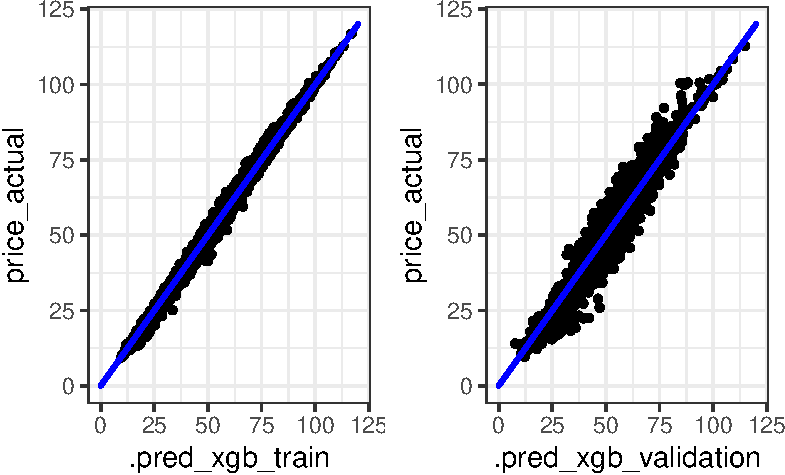
\includegraphics{Analytics_Report_files/figure-pdf/plotXgb-1.pdf}

This model is even better than the random forest model, and this can be
seen in the plot. Our predictions are getting closer and closer to the
line \(y = x\) and our RMSE has improved drastically.

\subsection{Model Assessment}\label{model-assessment}

\subsubsection{TSO Model}\label{tso-model}

The TSO model created by ENTSOE was used as a baseline for comparison
with our constructed models. This model had an RMSE of 13.25 on the
complete data set, indicating that 95\% of our predictions would fall
within plus or minus 2 RMSEs, about \$26. This is quite bad as the
electricity prices were generally in the \$50 or \$60 range. We greatly
improve upon this in our constructed models.

\subsubsection{Linear Regression Model}\label{linear-regression-model-1}

The linear regression model was built using hyper parameter tuning. The
best model had a mixture of 1.0 and a penalty of 0.0059948. This model
had an RMSE of 10.28 on the training data, and 10.22 on the validation
data. This RMSE is already quite a bit better than the TSO model, but
plots of our predictions compared to the true values indicate that the
model can still be improved. While linear regression models might not
give us the most accurate predictions for such complex relationships in
the real world, their interpretability is unmatched by other model
classes.

Let's look at our estimates for our linear regression model.

\begin{Shaded}
\begin{Highlighting}[]
\NormalTok{lin\_reg\_fit }\SpecialCharTok{|\textgreater{}}
  \FunctionTok{tidy}\NormalTok{() }\SpecialCharTok{|\textgreater{}}
  \FunctionTok{kable}\NormalTok{() }\SpecialCharTok{|\textgreater{}}
  \FunctionTok{kable\_styling}\NormalTok{()}
\end{Highlighting}
\end{Shaded}

\begin{longtable*}[t]{lrr}
\toprule
term & estimate & penalty\\
\midrule
(Intercept) & 5.4796101 & 0.0059948\\
generation\_biomass & 0.0252219 & 0.0059948\\
generation\_fossil\_brown\_coal\_lignite & -0.0008337 & 0.0059948\\
generation\_fossil\_coal\_derived\_gas & 0.0000000 & 0.0059948\\
generation\_fossil\_gas & 0.0008796 & 0.0059948\\
\addlinespace
generation\_fossil\_hard\_coal & 0.0018800 & 0.0059948\\
generation\_fossil\_oil & -0.0015470 & 0.0059948\\
generation\_fossil\_oil\_shale & 0.0000000 & 0.0059948\\
generation\_fossil\_peat & 0.0000000 & 0.0059948\\
generation\_geothermal & 0.0000000 & 0.0059948\\
\addlinespace
generation\_hydro\_pumped\_storage\_consumption & -0.0026821 & 0.0059948\\
generation\_hydro\_run\_of\_river\_and\_poundage & 0.0050756 & 0.0059948\\
generation\_hydro\_water\_reservoir & 0.0001605 & 0.0059948\\
generation\_marine & 0.0000000 & 0.0059948\\
generation\_nuclear & -0.0001249 & 0.0059948\\
\addlinespace
generation\_other & 0.0251382 & 0.0059948\\
generation\_other\_renewable & 0.2800691 & 0.0059948\\
generation\_solar & 0.0000000 & 0.0059948\\
generation\_waste & -0.0169519 & 0.0059948\\
generation\_wind\_offshore & 0.0000000 & 0.0059948\\
\addlinespace
generation\_wind\_onshore & 0.0000000 & 0.0059948\\
forecast\_solar\_day\_ahead & 0.0003795 & 0.0059948\\
forecast\_wind\_onshore\_day\_ahead & 0.0001493 & 0.0059948\\
total\_load\_forecast & 0.0001215 & 0.0059948\\
hour\_of\_day & 0.1306729 & 0.0059948\\
\addlinespace
month\_of\_year\_01 & 12.4060470 & 0.0059948\\
month\_of\_year\_02 & 6.1403905 & 0.0059948\\
month\_of\_year\_03 & -7.5809313 & 0.0059948\\
month\_of\_year\_04 & 4.8760670 & 0.0059948\\
month\_of\_year\_05 & 0.4609942 & 0.0059948\\
\addlinespace
month\_of\_year\_06 & 0.1563603 & 0.0059948\\
month\_of\_year\_07 & 1.6031846 & 0.0059948\\
month\_of\_year\_08 & 2.1259401 & 0.0059948\\
month\_of\_year\_09 & 1.5112374 & 0.0059948\\
month\_of\_year\_10 & -1.0475535 & 0.0059948\\
\addlinespace
month\_of\_year\_11 & 0.9580279 & 0.0059948\\
\bottomrule
\end{longtable*}

Our biggest contributors to our linear regression model seem to be from
the \texttt{month\_of\_year} column, which is quite interesting. This
indicates that day ahead electrical prices may be more dependent on the
time of year, rather than the load forecast or current generation
statistics.

\subsubsection{Random Forest Model}\label{random-forest-model-1}

The random forest model was built using hyper parameter tuning and took
nearly 45 minutes to tune. The best model had an RMSE of 1.77 on the
training data, and 4.12 on the validation data. This is significantly
better than both the linear regression and TSO models. We can now make
accurate predictions within plus or minus \$8 of the true price.

\subsubsection{Extreme Gradient Boosting
Model}\label{extreme-gradient-boosting-model-1}

The extreme gradient boosting model was built using hyper parameter
tuning and took 23 minutes to tune. The best model had an RMSE of 0.99
on the training data, and 3.44 on the validation data. This is even
better than the random forest model. This model can now make accurate
predictions within plus or minus \$7 of the true price. This model has
met the limitations of accuracy for the way our model was built. Further
accuracy could be attained by increasing the number of cross validation
folds and the number of levels in the parameter tuning step, however
this would greatly increase the time required to build the best model.

\subsection{Conclusion}\label{conclusion}

By effectively constructing models to predict power prices one day ahead
of time, this project greatly improved the baseline TSO model. The
linear regression model's simplicity limited its ability to capture the
complex relationships in energy markets, with an RMSE of 10.22 on the
validation data, but its interpretability is much better than that of
the random forest and extreme gradient boosting models.

The performance of other model classes, such as random forest and
extreme gradient boosting, was considerably better. On the validation
data, the extreme gradient boosting model achieved an RMSE of 3.44.
Because of its ability to predict prices within a range of plus or minus
\$7, it is a reliable tool for real world applications. The random
forest model was still quite good, but its performance could not match
that of the extreme gradient boosting model.

There are still challenges with the project even with successful models.
Our ability to improve model construction was limited by the time needed
for cross validation and hyper parameter tuning. Also, model classes
other than linear regression models provide great predictive power, but
at the cost of interpretability.

These results have important implications for industrial consumers,
energy producers, and grid operators. Predicting prices accurately one
day in advance allows for more effective resource allocation, reduces
the risk of fluctuations in renewable energy, and enhances grid
stability.

\subsection{References}\label{references}

{[}1{]}``Hourly energy demand generation and weather,'' www.kaggle.com.
https://www.kaggle.com/datasets/nicholasjhana/energy-consumption-generation-prices-and-weather

{[}2{]}OpenAI, ``ChatGPT,'' ChatGPT, 2024. https://chatgpt.com/




\end{document}
